%\setchapterpreamble[u]{\margintoc}
\chapter{Simulation, fusion and analysis of sensor data}
\labch{context}
\label{sec:context_rs}

The previous chapter presented the fundamentals of Remote Sensing which are required for this dissertation, including the notion of images, point clouds and widespread active and passive sensing tools. Different products are the result of these sensors, whereas data ought to be kept in a compact way for subsequent analyses. Hence, pixels from 2D maps, or points from 3D point clouds, are required to have a stack-based representation from each one of the available images. Figure \ref{fig:available_spectra} summarizes which parts of the spectra are available and which sensors provide this kind of information. Based on previous fundamental concepts, the state-of-the-art concerning the fusion of heterogeneous data, simulation and analysis are following presented.

\begin{figure}[ht]
	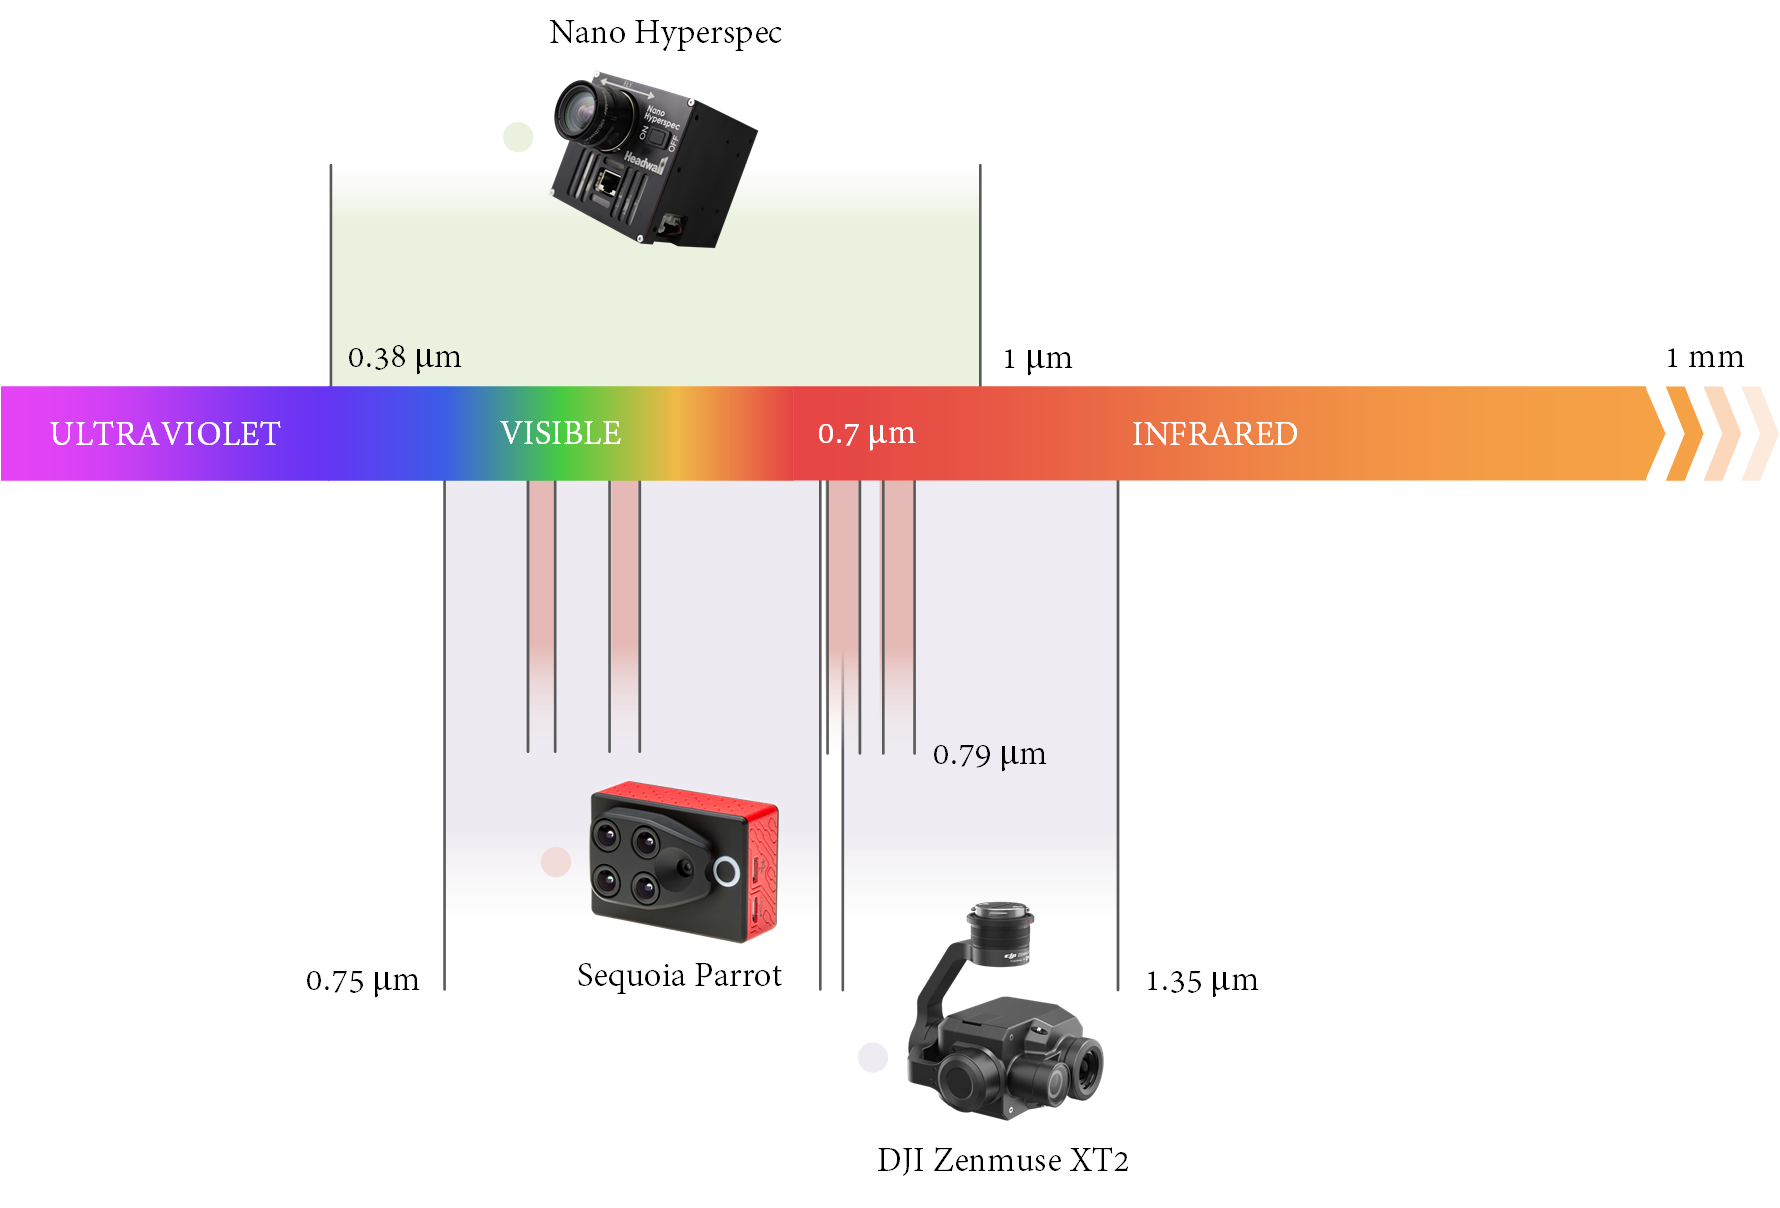
\includegraphics[width=.9\linewidth]{figs/context/spectra_devices.png}
	\caption{Available spectra from three different devices utilized for collecting \acrshort{uas}-based imagery. }
    \label{fig:available_spectra}
\end{figure}

This section is structured as follows. First, the fusion of images and point clouds is explored to match pairs of images, point clouds or images and point clouds. Rather than fusing visible imagery, which is the foundational core of photogrammetry, the focus here is on the fusion of visible imagery and other data sources. Then, the augmentation of remotely collected datasets is explored to generate point clouds from metropolitan and rural environments. Finally, the previously fused and generated data is applied to several case studies: the planning of scans in indoor scenarios, the phenotyping of grapevines and the inspection of archaeological sites in seek of buried remains.

\section{Fusion of information}

\subsection{Motivation}

The content of this section is principally obtained from the manuscript \textbf{"Remote sensing image fusion on 3D scenarios: A review of applications for agriculture and forestry"}. Although the aim of this publication was to revise work on the fusion of data for agriculture and forestry, only a few works related to this topic achieved 3D reconstruction with their own pipeline. Instead, most studies coped with 2D and 3D reconstruction using third-party software. Therefore, the domain of application was enlarged and a discussion was established for every revised methodology about the degree of applicability to agriculture and forestry areas.

The volume of remote sensing data is rapidly increasing and many real-world scenarios are currently being replicated by the generation of virtual models in 3D. The multi-source data integration and the 3D representation of surveyed areas is a hot research topic in the field of geoscience and remote sensing and has attracted the attention of both industry and academia. Focusing on natural and environmental areas, it has many prospective applications in smart agriculture \cite{jurado_multispectral_2020, padua_vineyard_2019, poblete_discriminating_2021}, forestry and nature preservation \cite{almeida_monitoring_2021, guimaraes_forestry_2020, heckel_predicting_2020, schiefer_mapping_2020} and monitoring \cite{maimaitijiang_crop_2020}. Initially, the acquisition of remote sensing data required costly sensors mounted on complex platforms. Likewise, the surveying procedure and data processing were labour-intensive and time-consuming. Observed scenarios were mainly represented in 2D maps and orthophotos, after applying manual processes to correct the image distortion \cite{vong_how_2021}. In this field, significant advances have been achieved by the development of efficient methodologies for data acquisition and processing, as well as the production of new sensor capabilities and aerial platforms. Accordingly, extensive research is currently being carried out focusing on multi-source data fusion and image mapping on 3D models.

In this context, the proliferation of \acrshort{uas} as versatile and cost-efficient platforms to acquire multi-source data has enabled the detailed characterization of large scenarios, even with difficult accessibility. Undoubtedly, \acrshort{uas} technology plays an important role in multidisciplinary research benefitting from unprecedented temporal, spatial and spectral resolution, acquired from multiple perspectives in a non-intrusive way.

Although data fusion can be performed over pairs of images, most applications use this as a first step towards approaching 3D reconstructions. From here, primitives from 3D representations, obtained with a single data source, are easily back-projected to another data source. Thus, stack-based representations from image matching also lead to point clouds with multiple layers. Besides the benefits of 3D models in visual inspections, these are significantly more valuable when combined with \acrshort{rgb}, multispectral, hyperspectral and thermal data. The fusion of these data and 3D geometry depicting natural and artificial surfaces brings a deep knowledge of our environment. Figure \ref{fig:scopus_point_clouds} offers a vision of how 3D modelling has been gaining interest in data sources beyond the visible spectral range. The Scopus searches were the following: $(p_1 \lor p_2 ... \lor p_n) \land ((\textit{point} \hspace{1mm} \land \hspace{1mm} \textit{cloud}) \lor (\textit{3D} \hspace{1mm} \land \hspace{1mm} \textit{modelling}))$, with $p_i$ being different names that identify a data source (e.g., visible and \acrshort{rgb}).

\begin{figure}[ht]
    \centering
    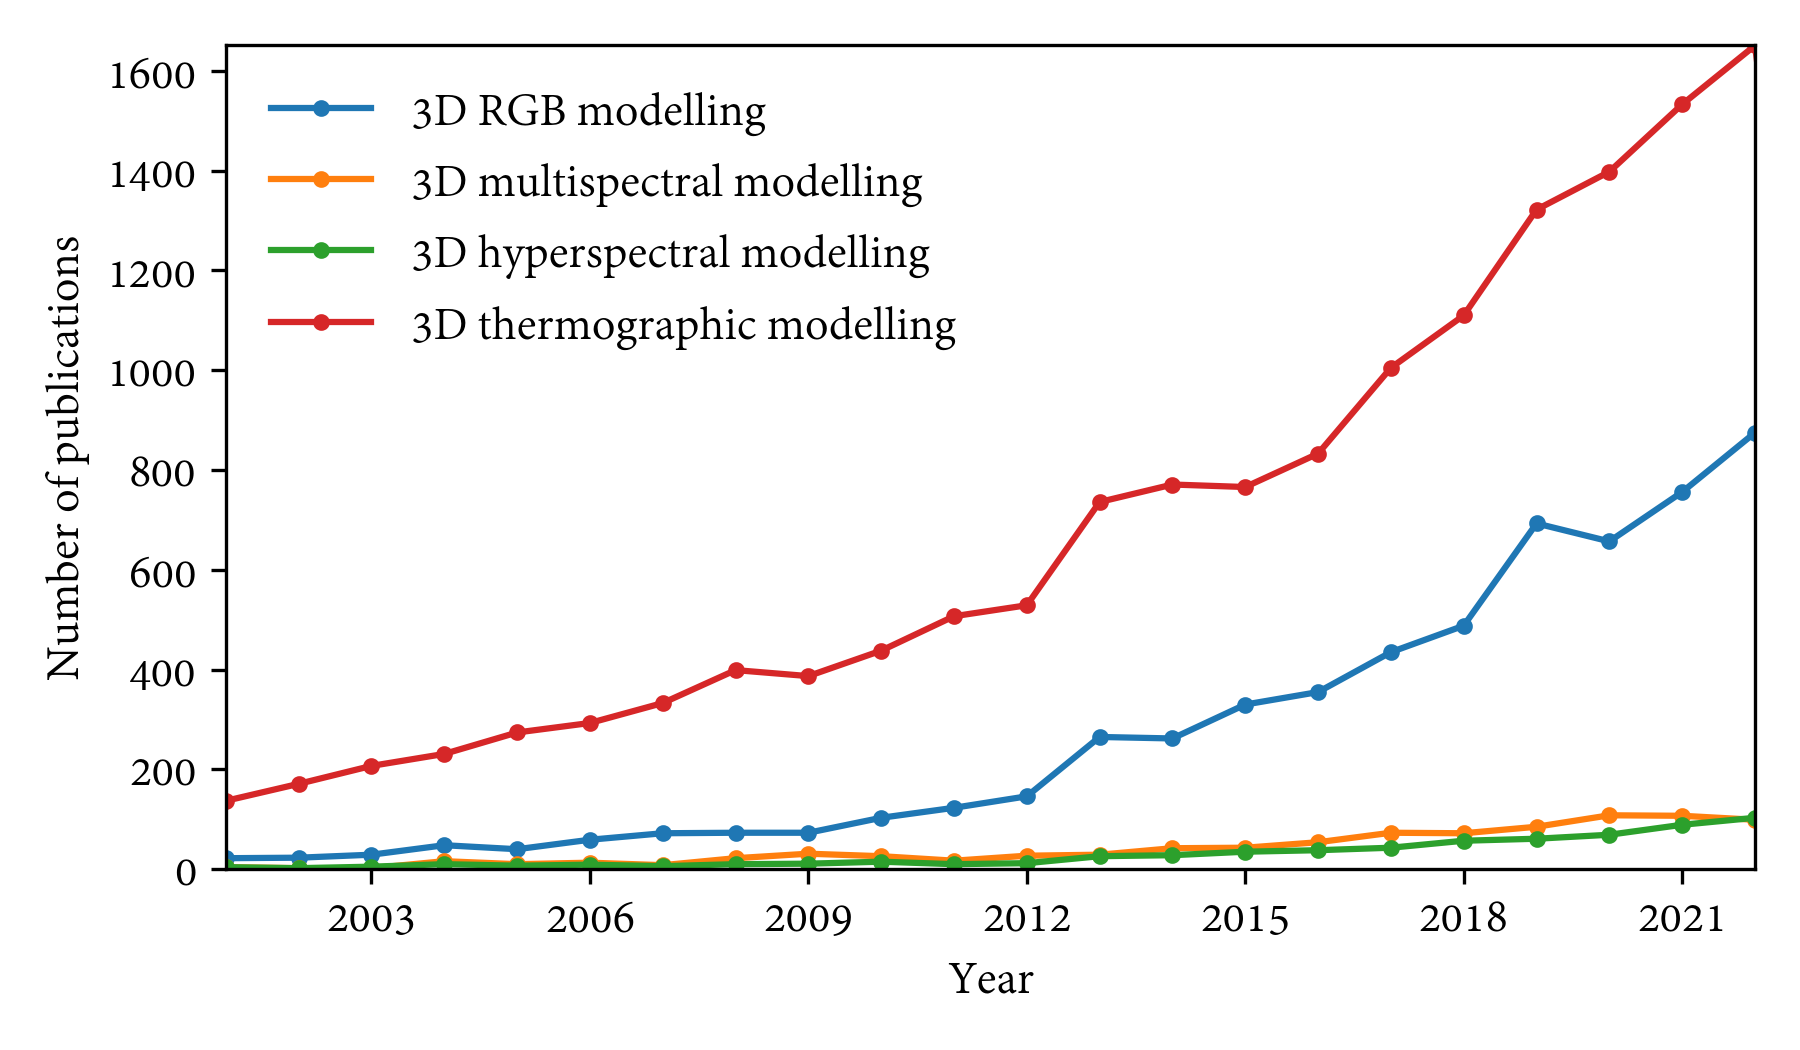
\includegraphics[width=\linewidth]{figs/context/3d_modelling.png}
	\caption{Number of publications related to visible, multispectral, hyperspectral and thermographic 3D modelling, from 2000 to the current year. }
	\label{fig:scopus_point_clouds}
\end{figure}

The integration of multiple data sources, in combination with 3D reconstructions, is still challenging since each dataset is obtained with a different mechanism (global or rolling shutter, push broom sensors, etc.), intrinsic and extrinsic parameters, distortion and resolution. Therefore, fusing multiple datasets is not trivial and demands high computational efforts that can be alleviated with \acrshort{gpgpu}. In the following subsections, the main contributions to the fusion of visible, thermographic, multispectral and hyperspectral data are summarized. First, the fusion of 2D data is reviewed and then, the combination of imagery and point clouds is revised. Both sections are split into works related to thermal, multispectral and hyperspectral data. 

\subsection{Image matching}

\subsubsection{Thermal infrared imaging}

Consumer-grade \acrshort{ir} cameras are not prohibitive, at the expense of having lower resolution and a higher number of defects. Sledz et al. \cite{sledz_thermal_2018} reported several sources of noise causing \acrshort{ir} images to have a blurred and smoothed-out appearance. Among these, environmental conditions and non-uniformity of focal plane arrays (\acrshort{fpa}) were highlighted \cite{javadnejad_photogrammetric_2020}. Furthermore, the radiation of a surface is captured by several detector elements, as energy spreads to the surroundings \cite{vollmer_infrared_2017}. \acrshort{uas} platforms are less affected by the attenuation from energy dispersion and atmospheric absorption, though this is a well-known problem in thermography \cite{gonzalez_thermal_2019, vollmer_infrared_2017, quattrochi_thermal_1999}.

Amongst works addressing matching visible and thermal imagery, only a few consider that both data sources are perfectly overlapped as collected \cite{hou_fusing_2021, stojcsics_high_2018}. However, this scenario is not frequent; instead, visible and thermal imagery record slightly different areas of interest, even for images co-acquired by dual devices. This is caused by minor differences in triggering timestamps, the platform's movement and the device calibration, which may degrade over time. 

The most frequent approaches for \acrshort{ir} image registration are depicted in Figure \ref{fig:fusion_data_03}. One of the main concerns is the selection of the most appropriate feature descriptor. The reviewed literature shows a higher preference for edge detection algorithms, such as Canny and Sobel operators \cite{hoegner_3d_2016, hoegner_evaluation_2016}, over conventional feature descriptors, including the Scale-invariant feature transform (\acrshort{sift}), Speeded-Up Robust Features (\acrshort{surf}) and Oriented FAST and rotated BRIEF (\acrshort{orb}) (Figure \ref{fig:feature_descriptors}). In this regard, Hoegner et al. \cite{hoegner_evaluation_2016} enhanced the edge detection by solely conserving prominent edges with the Hough transform \cite{hoegner_evaluation_2016}. However, edge detection algorithms are not as appropriate for forestry and rural scenarios, as depicted in Figure \ref{fig:feature_detection}. Previous work has also coped with image matching on the frequency domain, with the aim of handling nonlinear colourimetric differences between visible and \acrshort{ir} imagery. Lin et al. \cite{lin_fusion_2019} implemented the Radiance Invariant Feature Transform (\acrshort{rift}) \cite{lin_fusion_2019}, followed by a suppression of mismatches with Random Sample Consensus (\acrshort{ransac}).

From here, projecting \acrshort{ir} imagery in 3D reconstructions is trivial; 3D points are efficiently projected into \acrshort{rgb} images, which have already been matched with thermography. Figure \ref{fig:fusion_data_03} illustrates the image-matching algorithms and how these help in the later 3D reconstructions. 

\begin{figure*}[ht]
	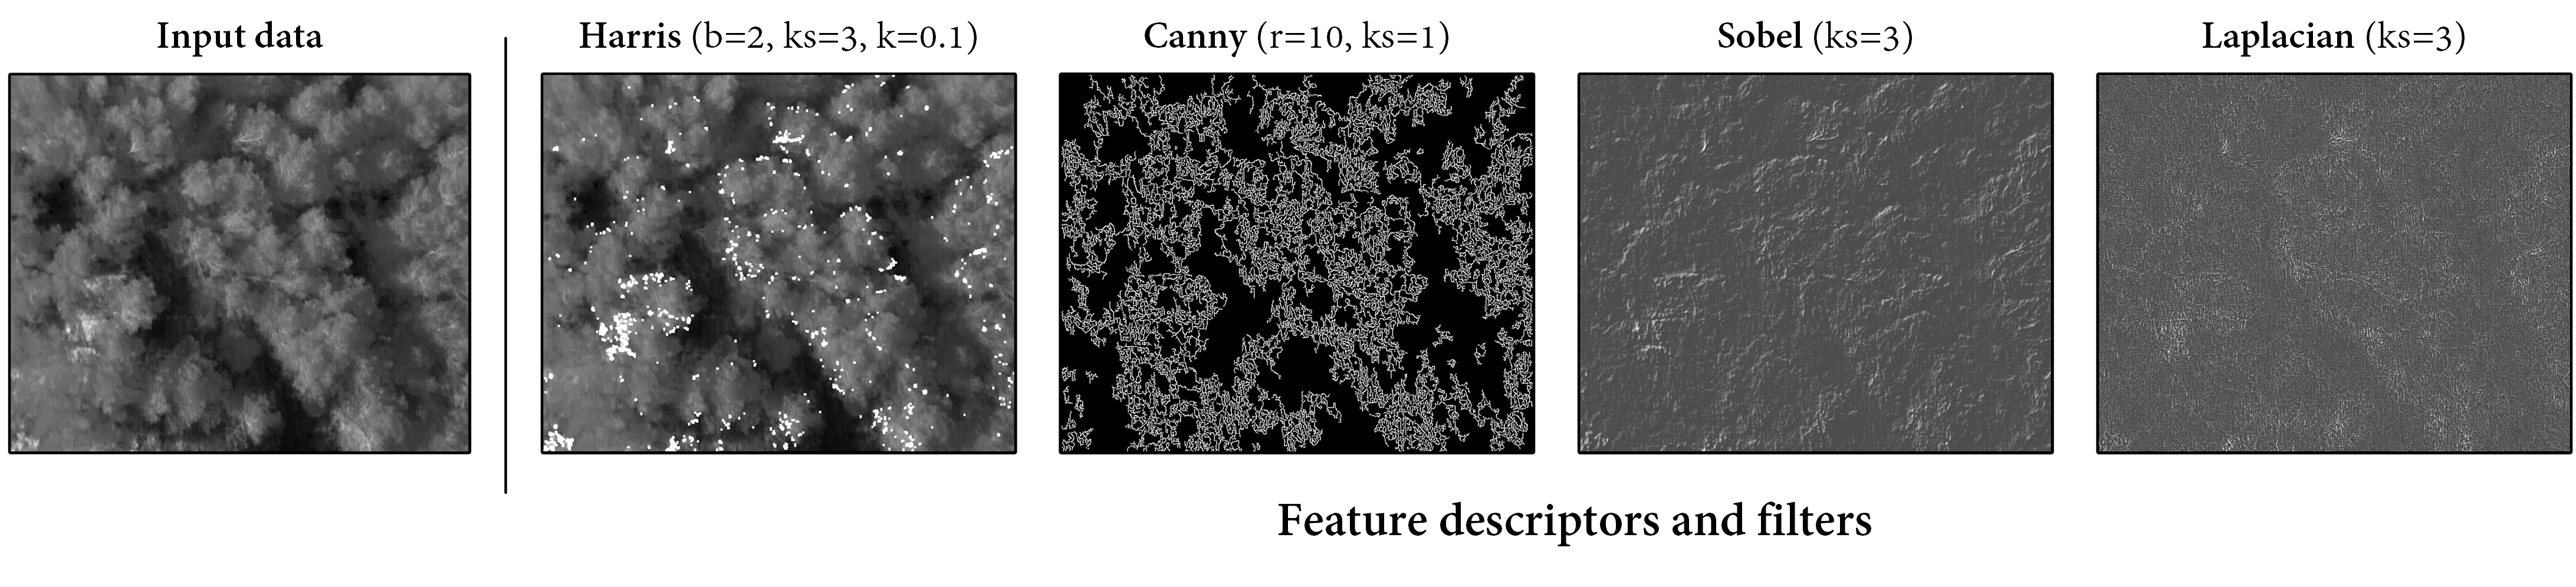
\includegraphics[width=\linewidth]{figs/context/feature_detection.png}
	\caption{Comparison of edge-based feature descriptors frequently used in image registration algorithms. These are less likely to work for vegetation as no relevant features are found. $\textit{ks}$ refers to kernel size, the ratio is presented as $\textit{r}$, and $\textit{k}$ is a free parameter on the Harris detector. The brightness of the two first images is increased to improve the visualization.}
    \label{fig:feature_detection}
\end{figure*}

Instead of using colourimetric data, other studies have proposed a calibrated system with multiple devices. Thermographic imagers are frequently combined with \acrshort{rgb} cameras \cite{javadnejad_photogrammetric_2020, landmann_multimodal_2019, adan_fusion_2017} and \acrshort{lidar} \cite{adan_fusion_2017, hoegner_fusion_2018}. The calibration of dual-sensor systems is performed by estimating the translation (lever-arm) and rotation (boresight) matrices that represent how these sensors correlate (see Figure \ref{fig:fusion_data_04}). Calibration is frequently performed by identifying features visible in several images, either following a supervised or semi-supervised approach. However, the calibration of systems with multiple sensors was proven to perform worse in inexpensive, consumer-grade thermal cameras \cite{javadnejad_photogrammetric_2020}. Constructing a checkerboard calibration panel and marking features on it is particularly tough using \acrshort{ir} data \cite{javadnejad_photogrammetric_2020} since it lacks sharp edges. However, these systems with multiple devices have the advantage of rapidly fusing 2D and 3D data simultaneously once calibrated.

\begin{figure*}[ht]
	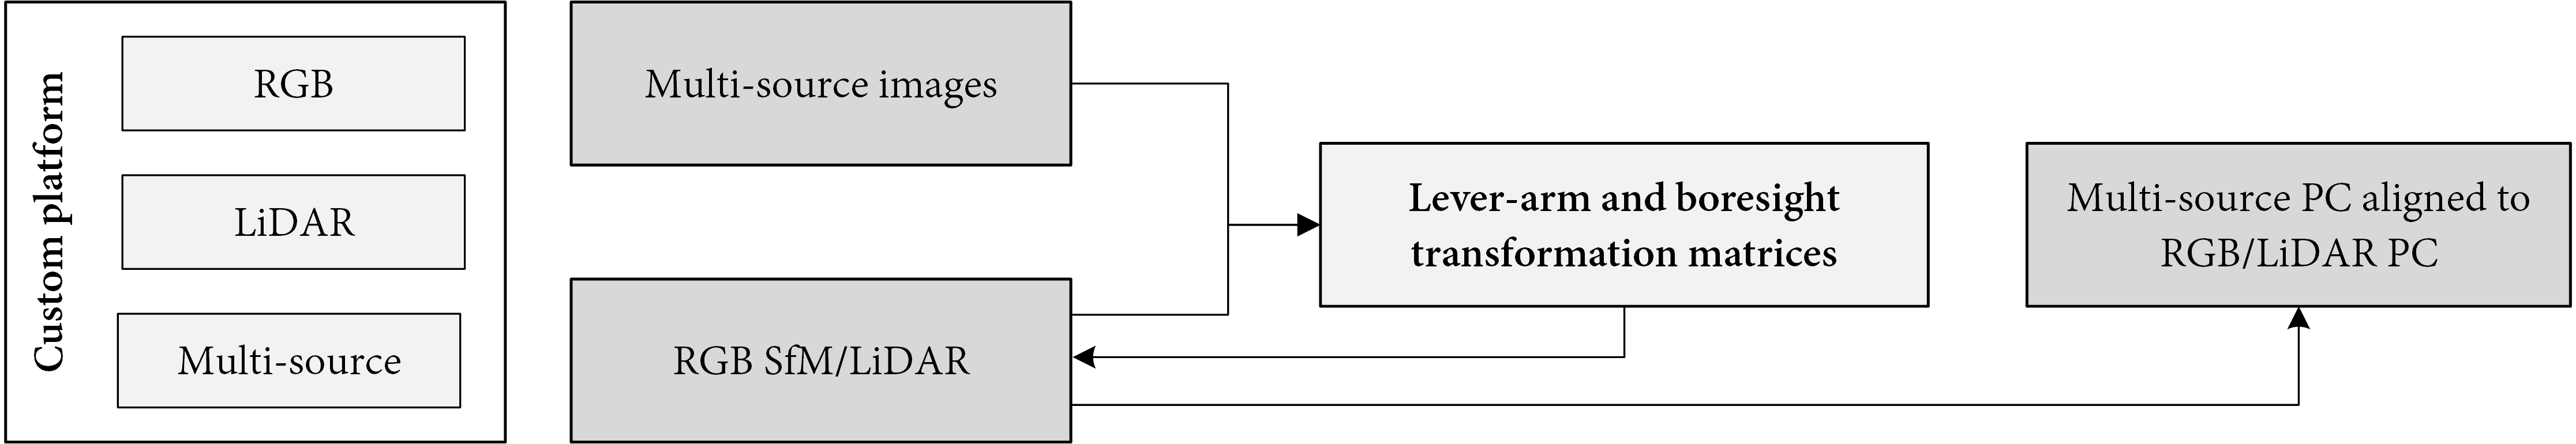
\includegraphics[width=\linewidth]{figs/context/fusion_04.png}
	\caption{Systems with multiple sensors are calibrated with the aim of projecting multiple data sources into a single coordinate system.}
    \label{fig:fusion_data_04}
\end{figure*}

\subsubsection{Multispectral imaging}

Unlike \acrshort{ir}, multispectral datasets are composed of several bands in the visible and infrared wavelengths. These bands are more likely to not record the exact same area of interest, influenced by different positioning of lenses, the platform's movement and the calibration of each individual imager, which deteriorates over time. Shen et al. \cite{shen_multi-modal_2014} introduced an image-matching solution based on a descriptor measuring the degree of matching for every pixel. Other works used the orientation embedded in the image metadata to correct the misalignment \cite{jhan_band--band_2016}, and the error of these parameters was reduced with \acrshort{ransac} \cite{jhan_investigation_2017}. Similarly to \acrshort{ir} image-matching, the \acrshort{surf} \cite{sedaghat_high-resolution_2019} and \acrshort{sift} \cite{saleem_robust_2014} feature descriptors have also been applied to multispectral datasets. According to Tsai and Lin \cite{tsai_accelerated_2017}, the \acrshort{sift} method outperformed other algorithms in terms of quality of results and efficiency.

\begin{figure}[ht]
	\includegraphics[width=\linewidth]{figs/context/feature_extraction.png}
	\caption{Comparison of two traditional feature descriptors and matching algorithms: \acrshort{sift} and  \acrshort{orb}. In this example, both are used to match multi-view sequences of the same scene.}
    \label{fig:feature_descriptors}
\end{figure}

\subsubsection{Hyperspectral imaging}

Hyperspectral sensors collect the light intensity in a large number of contiguous spectral bands, typically ranging from a few tens to several hundred. Every pixel stores the spectral response of one or multiple materials, thus helping to understand images and monitor scenarios. \acrshort{hsi} comprises several scan geometries, already explained in Section \ref{sec:fundamentals_optical_imaging_geometry}, although the vast majority of works are based on the push broom technology (see Figure \ref{fig:hyper_scan_geometry}). Push broom sensors include a set of 2D detectors that simultaneously sample all the points along a line. The area of interest is surveyed by translating the platform in the direction orthogonal to such a line. This scanning technology enables the simultaneous acquisition of every wavelength in a pixel, thus facilitating and reducing the post-processing of hypercubes. It is also worth noting that the type of sensor greatly affects field operations, processing performance and the quality of the final product \cite{adao_hyperspectral_2017}. 

With this in mind, the main objective of fusing hyperspectral data with other data sources is to correct the geometric distortions, and therefore, the other data source is the reference without geometric errors. In this regard, Jurado et al. \cite{jurado_efficient_2021} proposed a method for matching hyperspectral and high-resolution \acrshort{rgb} imagery. Hyperspectral swaths were split into smaller fragments, and the \acrshort{orb} feature descriptor was used to find common features. From here, it was estimated whether the resulting transformation matrix was feasible or not by measuring the distance of control points in hyperspectral (after projection) and \acrshort{rgb} imagery. Otherwise, a smaller partition of the swath was used until a stable alignment was achieved or the current fragment could be further split. Previously, Angel et al. \cite{angel_automated_2020} aligned hyperspectral and \acrshort{rgb} images by applying \acrshort{surf} and discarding mismatches with a variant of \acrshort{ransac}, Maximum Likelihood Sample Consensus (\acrshort{mlsac}). Also recently, Akhoundi Khezrabad et al. \cite{akhoundi_khezrabad_new_2022} avoided the use of \acrshort{gcp}s by simultaneously recording a video together with hyperspectral data. \acrshort{sift}, \acrshort{ransac} and Spectral Angle Mapper (\acrshort{sam}) were applied to the geometric correlation. Note that \acrshort{sam} helps to discard mismatches since it measures how similar are two spectral signatures regardless of their scale.

\subsection{3D reconstructions}

\subsubsection{Thermographic imaging}

The majority of outdoor \acrshort{ir} datasets come from \acrshort{uas} platforms, despite terrestrial and indoor collections also being frequent. Lin et al. \cite{lin_fusion_2019} and Stojcsics et al. \cite{stojcsics_high_2018} collected \acrshort{ir} data from a hand-held camera, whereas Zhu et al. \cite{zhu_fusion_2021} recorded both \acrshort{ir} and \acrshort{lidar} from a vehicle coupled with multiple sensors. Adán et al. \cite{adan_towards_2020} used a robotic platform to autonomously navigate and scan indoor environments. Previous work also exploited the use of custom systems that are geometrically calibrated by describing the lever-arm between multiple sensors \cite{javadnejad_photogrammetric_2020, hoegner_fusion_2018}. This calibration is achieved by collecting multiple images depicting a known pattern, typically a checkerboard \cite{javadnejad_photogrammetric_2020} or landmarks with peculiar reflectivity \cite{adan_fusion_2017}. 

\begin{figure*}[ht]
	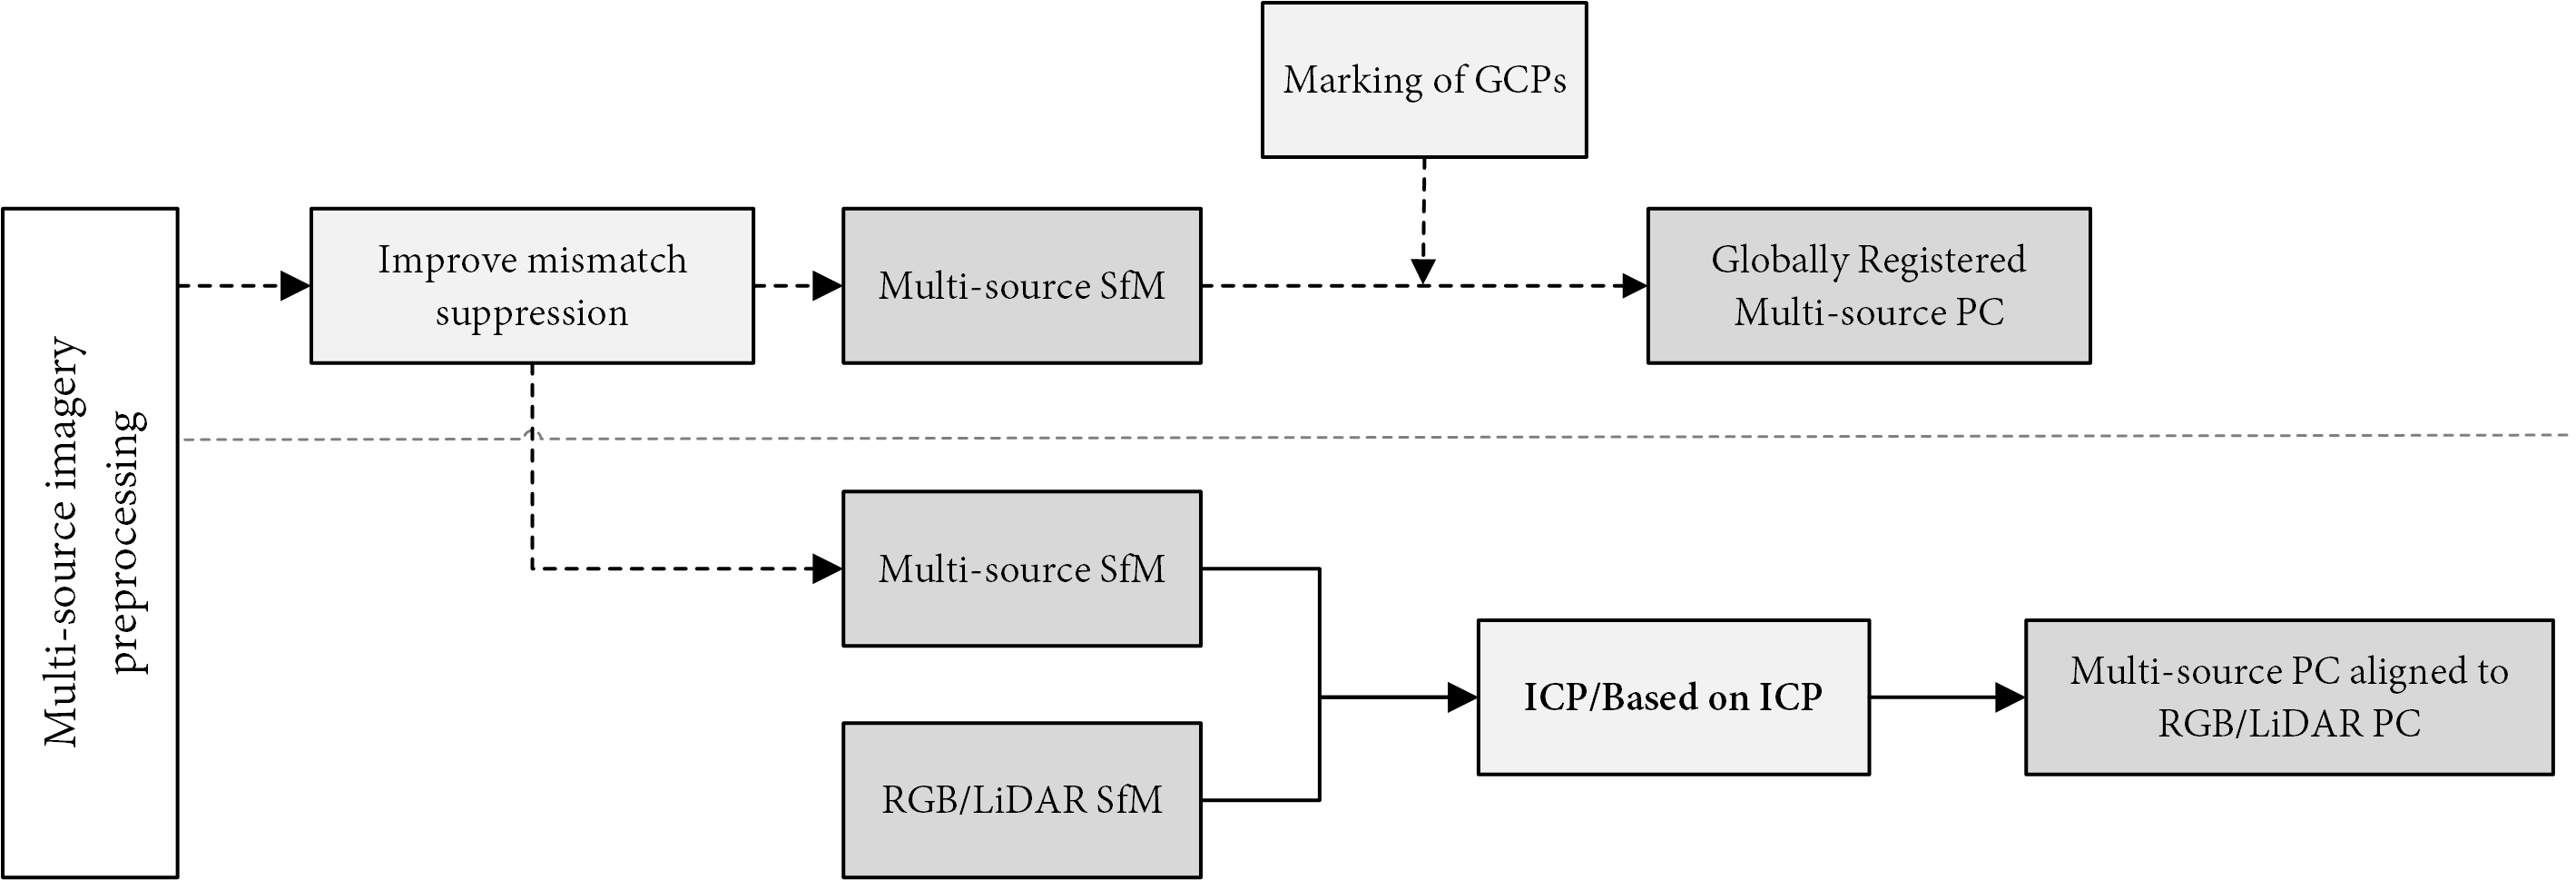
\includegraphics[width=\linewidth]{figs/context/fusion_01.png}
	\caption{Two different approaches for reconstructing 3D \acrshort{ir} models. First, \acrshort{sfm} is used over visible and \acrshort{ir} datasets, whereas the second procedure estimates the rigid transformation that aligns two point clouds. }
    \label{fig:fusion_data_01}
\end{figure*}

In spite of the low resolution of \acrshort{ir} imagery, previous work has extensively applied photogrammetry to reconstruct \acrshort{ir} point clouds \cite{dahaghin_precise_2021, dahaghin_3d_2019, gonzalez_thermal_2019, grechi_3d_2021, webster_three-dimensional_2018, sledz_thermal_2018, kniaz_thermal_2018, hoegner_mobile_2018, zheng_thermal_2020, guilbert_fusion_2020}. This paradigm is illustrated in Figure \ref{fig:fusion_data_01}. Among other factors, this approach is very frequent since \acrshort{sfm} is part of notable commercial and open-source software and thus is particularly easy to apply. Some of these third-party solutions are Pix4Dmapper \cite{zheng_thermal_2020}, Agisoft Metashape \cite{grechi_3d_2021, guilbert_fusion_2020, lin_fusion_2019, macher_combination_2019}, Autodesk Recap 360 \cite{lafi_3d_2017} and Zephyr \cite{maset_photogrammetric_2017, clarkson_thermal_2017}. Although photogrammetry is trivial to apply from third-party software, \acrshort{ir} imagery has defects and limitations that harden this process, for instance, on the retrieval of tie points during feature detection \cite{lin_fusion_2019}. Consequently, resulting point clouds are more likely to be scarce, less precise and more geometrically inaccurate due to noise, gaps and incorrectly estimated elevation \cite{kong_3-d_2018}. Photogrammetry is similarly problematic for environments showing repetitive patterns and uniform textures, e.g., buildings and vegetation \cite{lin_fusion_2019, jarzabek-rychard_supervised_2020}, even for other data sources. On the other hand, geometrical inaccuracies can be mitigated using \acrshort{gcp}s. However, the marking of \acrshort{gcp}s is more challenging in thermography due to the low resolution and colour contrast \cite{sledz_thermal_2018}. Still, previous work has explored the placement of \acrshort{gcp}s without further considerations to reconstruct \acrshort{ir} point clouds \cite{dahaghin_precise_2021, gonzalez_thermal_2019, zheng_thermal_2020, sledz_thermal_2018}. Boesch et al. \cite{boesch_thermal_2017} and Nishar et al. \cite{nishar_thermal_2016} overcome the limited visibility of \acrshort{gcp}s by using metal-coated materials with low emissivity, in contrast with the surrounding vegetation. In this regard, Figure \ref{fig:gcps_thermography} shows the poor visibility of non-metal-coated \acrshort{gcp}s when they are surrounded by vegetation (with similar radiation) instead of bare soil. 

\begin{figure*}[ht]
	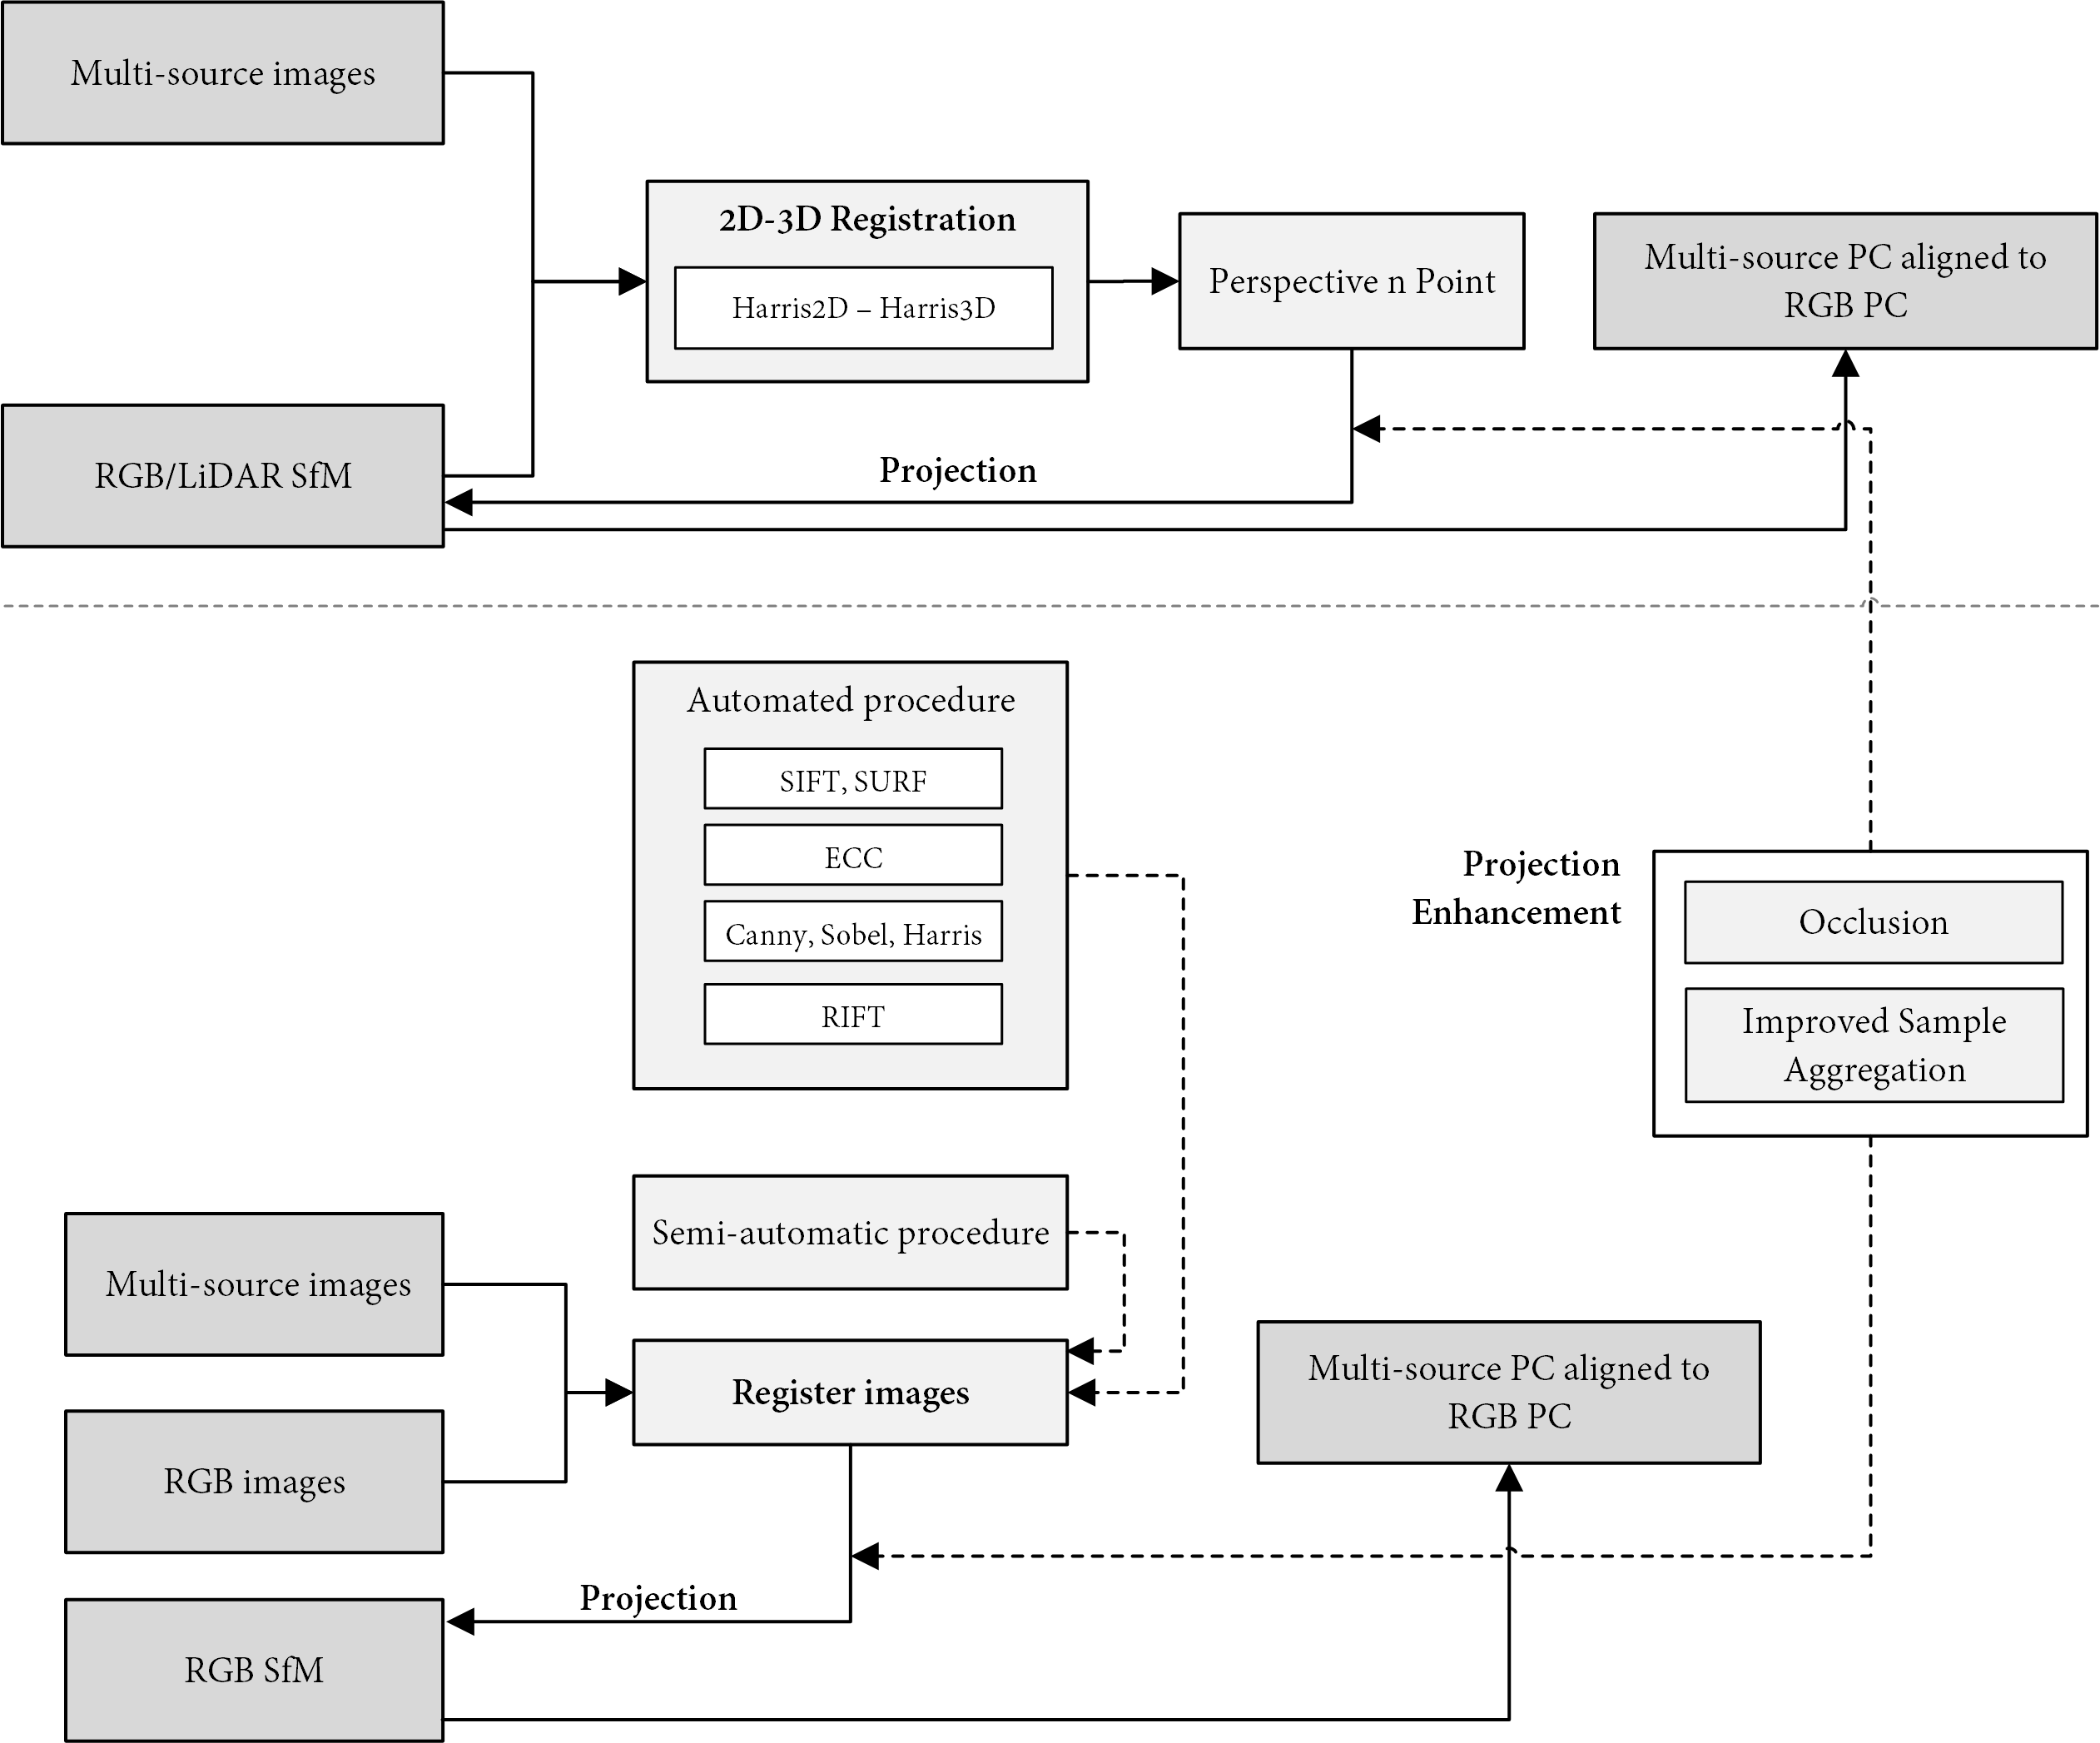
\includegraphics[width=\linewidth]{figs/context/fusion_03.png}
	\caption{Two different methods for reconstructing 3D point clouds. First, images are mapped into a baseline point cloud once 2D and 3D features are correlated and used to estimate pose parameters. In the second approach, features are only sought in 2D to compute the transformation matrix between \acrshort{rgb} imagery and other data source. }
    \label{fig:fusion_data_03}
\end{figure*}

\begin{figure}[ht]
	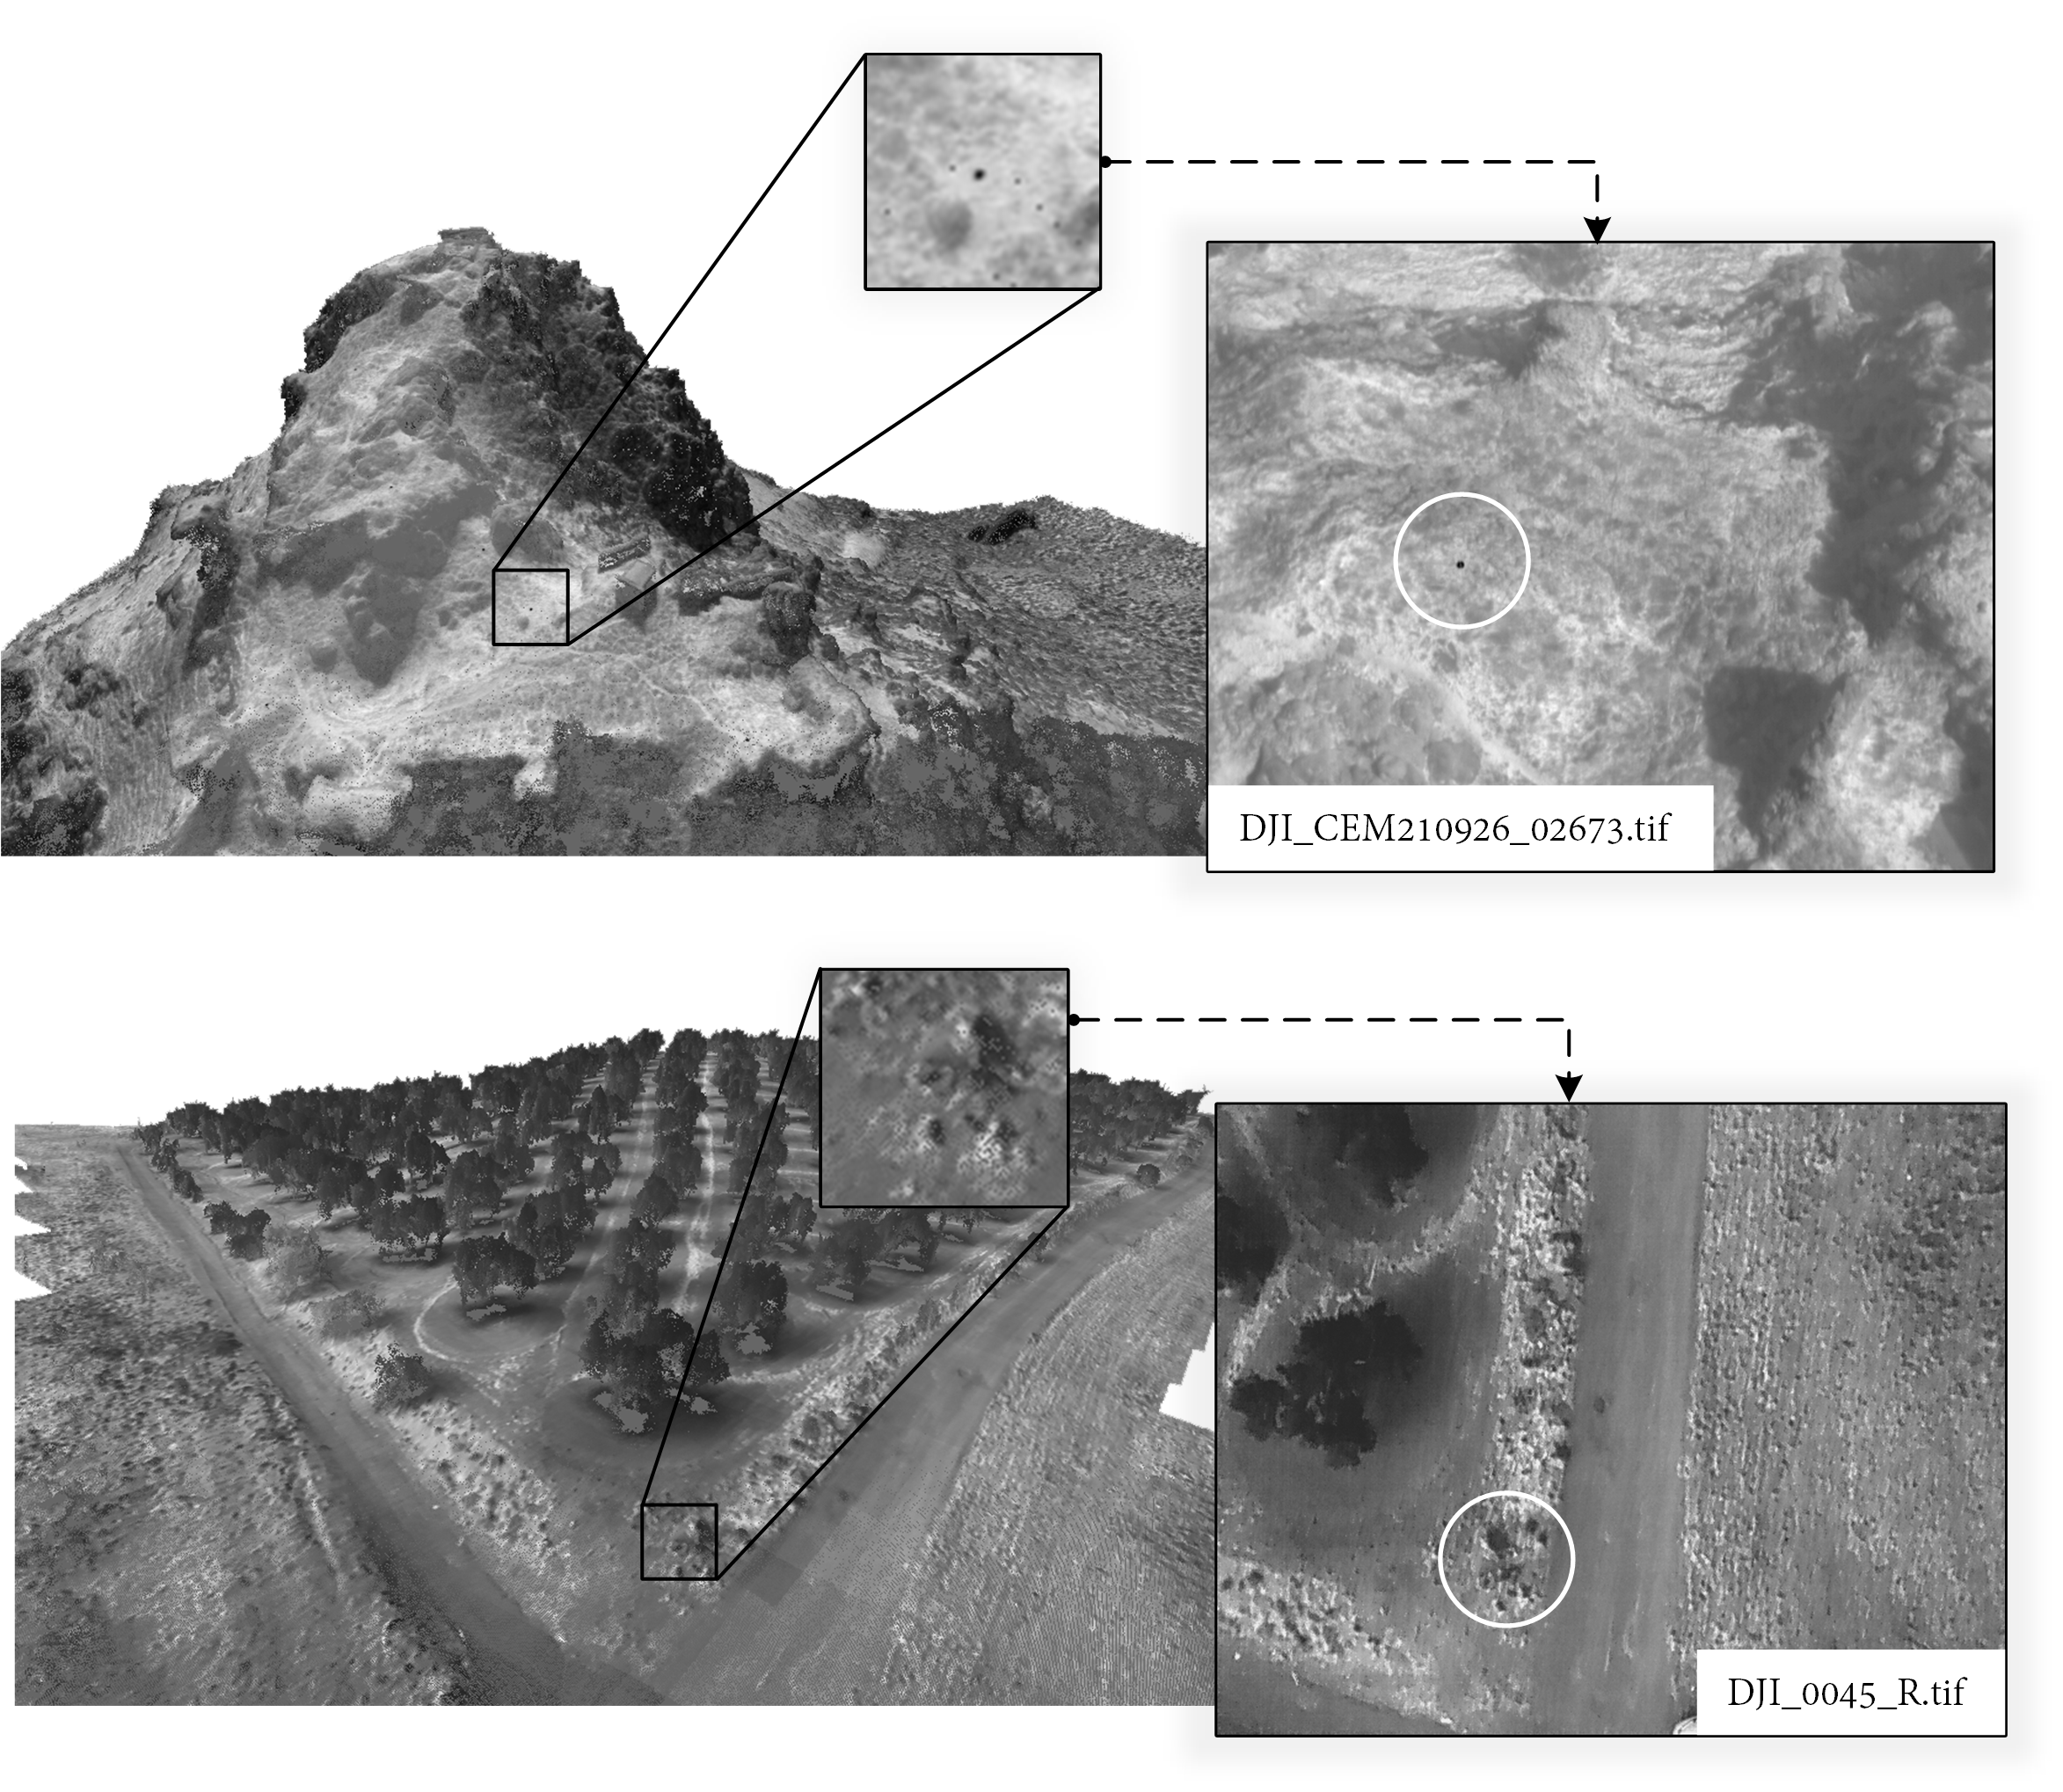
\includegraphics[width=\textwidth]{figs/context/gcps.png}
	\caption{Non-metal-coated \acrshort{gcp}s made of plastic under two different scenarios. \acrshort{gcp}s are barely noticeable in the second scenario since the surroundings have a similar temperature. In the first scenario, they are significantly more visible to the naked human eye since the surroundings are bare soil. }
    \label{fig:gcps_thermography}
\end{figure}

Another revised approach is to improve some of the stages of \acrshort{sfm} with the help of other data sources. For instance, the External Orientation Parameters (\acrshort{eop}) could be estimated from visible datasets that have larger dimensionality and higher accuracy \cite{jo_dense_2021}. Maes et al. \cite{maes_optimizing_2017} estimated the \acrshort{ir} camera parameters using the Brown-Conrady distortion model. The temperature was corrected by decoupling the influence of air temperature in multiple flights. Also, the image geopositioning was improved with the onboard \acrshort{gps} and Global Navigation Satellite System (\acrshort{gnss}). To overcome the limitations imposed by the \acrshort{sfm}'s keypoint detection, previous work has explored other algorithms aimed at extracting features and suppressing mismatches. In this regard, Kong et al. \cite{kong_3-d_2018} applied \acrshort{knn} to remove evident mismatches, followed by a modification of \acrshort{ransac} where the temperature was used to tell mismatches apart. 

Instead of only using \acrshort{ir} data, the fusion of several data sources, with one of them being \acrshort{ir}, has also been extensively investigated. \acrshort{rgb} images are typically the baseline since they help to reconstruct more dense and accurate 3D point clouds. Therefore, the vast majority of previous work projects \acrshort{ir} data over this baseline point cloud \cite{hosoi_estimating_2019, javadnejad_photogrammetric_2020}. Visible and thermal image matching has been traditionally performed using 2D and 3D feature descriptors, whereas mismatches are filtered out. Once two or more image datasets are aligned, these can be projected to 3D \acrshort{rgb} points. This approach is able to generate larger \acrshort{ir} point clouds by upsampling thermal data. 

The projection of \acrshort{ir} data into \acrshort{rgb} point clouds can also be achieved by mixing 3D products and thermal imagery by means of 3D feature descriptors. Following this approach, the Perspective n Point (\acrshort{pnp}) optimization has been solved by pairing 3D and 2D features, thus estimating the camera poses (see Figure \ref{fig:fusion_data_03}). Most of these features are extracted with edge-based operators, from which \acrshort{sift} and \acrshort{sift}3D stand out. However, these have been reported to identify insufficient key points and have been often exchanged by the Harris and Harris3D operators \cite{zhu_fusion_2021, zhu_direct_2019}. These are more robust and extract features that are less likely to appear in other locations within a single image. Instead of using the bare contours, Lin et al. \cite{lin_fusion_2019} used the edge intersections as key points. However, most of these methods for matching 2D and 3D features are not robust enough to work under most scenarios. Therefore, the feature matching has also been aided by human operators \cite{zhu_fusion_2021, zhu_direct_2019} or by restricting the search space with \acrshort{gps}/\acrshort{gnss} data, with \acrshort{ransac} helping to discard mismatches \cite{lin_fusion_2019}. 

Reconstructing thermal point clouds and aligning them with \acrshort{rgb} products is also tempting in spite of the differences concerning density and noise. The distance between both point clouds can be described with a transformation matrix, whose error can be minimized with the Iterative Closest Point (\acrshort{icp}). It returns a composite matrix involving translation, rotation, and optionally, scaling \cite{hoegner_mobile_2018, webster_three-dimensional_2018, clarkson_thermal_2017}. Rather than solely applying the \acrshort{icp} algorithm, the noise is firstly filtered out, followed by a coarse global registration with a rigid body transformation estimated using the camera poses \cite{truong_registration_2017}. Still, \acrshort{icp} can operate as a local registration that provides more fine-grained results. An alternative to \acrshort{icp} is Fast Global Registration (\acrshort{fgr}), which is proven to achieve better results with noisy datasets \cite{lin_fusion_2019}. Point clouds can also be registered by means of at least three \acrshort{gcp}s if they can be accurately marked \cite{dahaghin_3d_2019}. In addition, the use of \acrshort{icp} along with \acrshort{knn} has been investigated to assign \acrshort{ir} data to 3D \acrshort{rgb} points, with the outcome being a dense 3D model with upsampled thermal data. More recently, an rotation invariant descriptor that extracts features from icosahedral groups has been investigated \cite{wang_you_2022}.

\begin{marginfigure}[-3cm]
	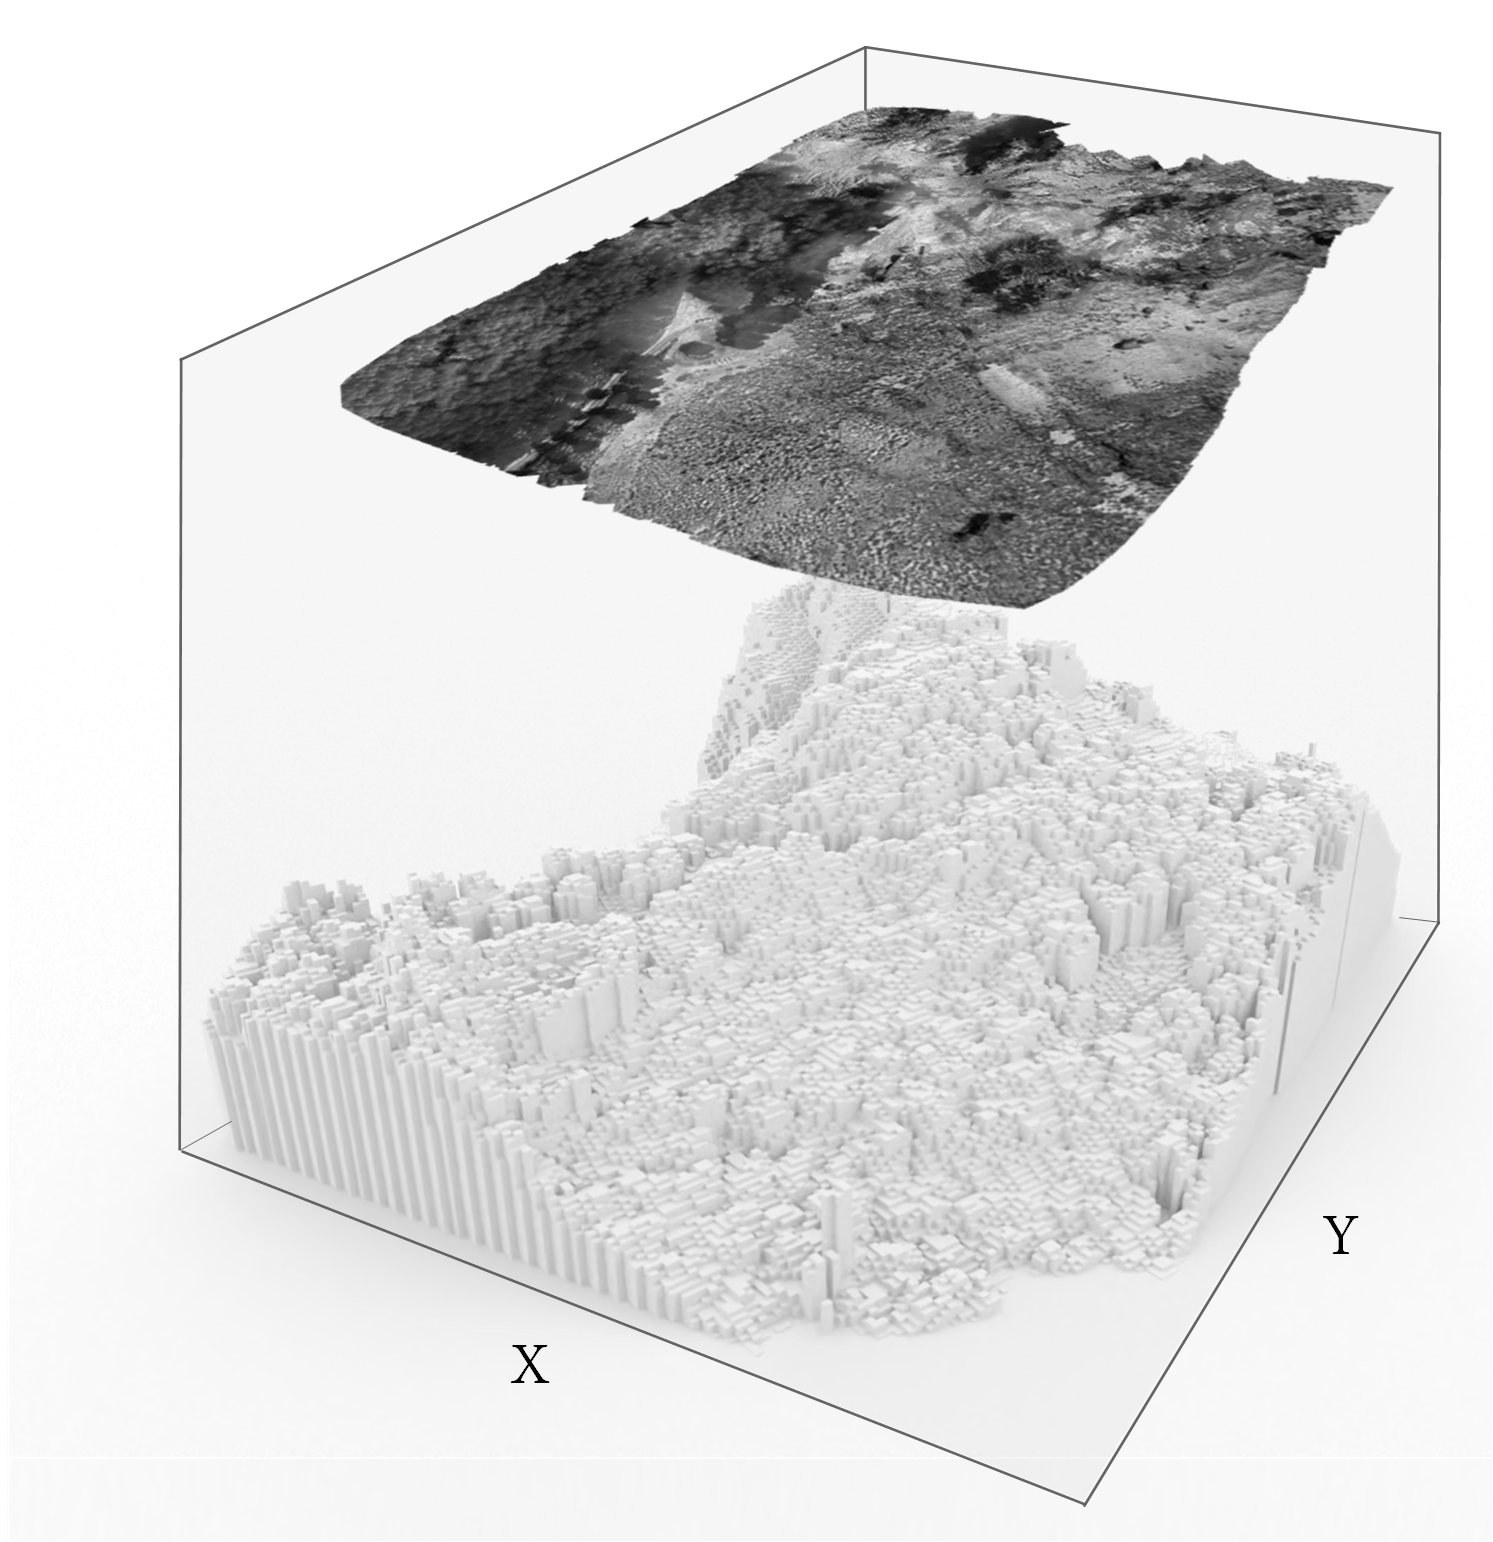
\includegraphics{figs/context/orthomosaic_projection.png}
	\caption{Projection of an orthomosaic over a 2.5D point cloud.}
	\label{fig:ortho_projection}
\end{marginfigure}
\acrshort{ir} 3D models can also be constructed by combining \acrshort{lidar} and visible point clouds with thermal maps in the same coordinate system (Figure \ref{fig:fusion_data_02}). Comba et al. \cite{comba_2d_2019} fused an \acrshort{rgb} point cloud with a thermal orthomosaic (Figure \ref{fig:ortho_projection}), whereas Adán et al. \cite{adan_towards_2020} combined \acrshort{lidar} results with 360-degree maps of \acrshort{ir} data. These studies generate a single thermal image with a limited resolution which is subsequently projected in a 3D model. The former approach obtains \acrshort{ir} heightfields (2.5D) \cite{juszczyk_wound_2021}, whereas the main drawback of the work of Adán et al. \cite{adan_towards_2020} is that some points lack \acrshort{ir} data as a result of foreground surfaces occluding background surfaces. This problem was mitigated by using a mobile scanning platform and joining multiple thermal point clouds using the platform odometry and the \acrshort{icp} algorithm. 

\begin{figure}[ht]
	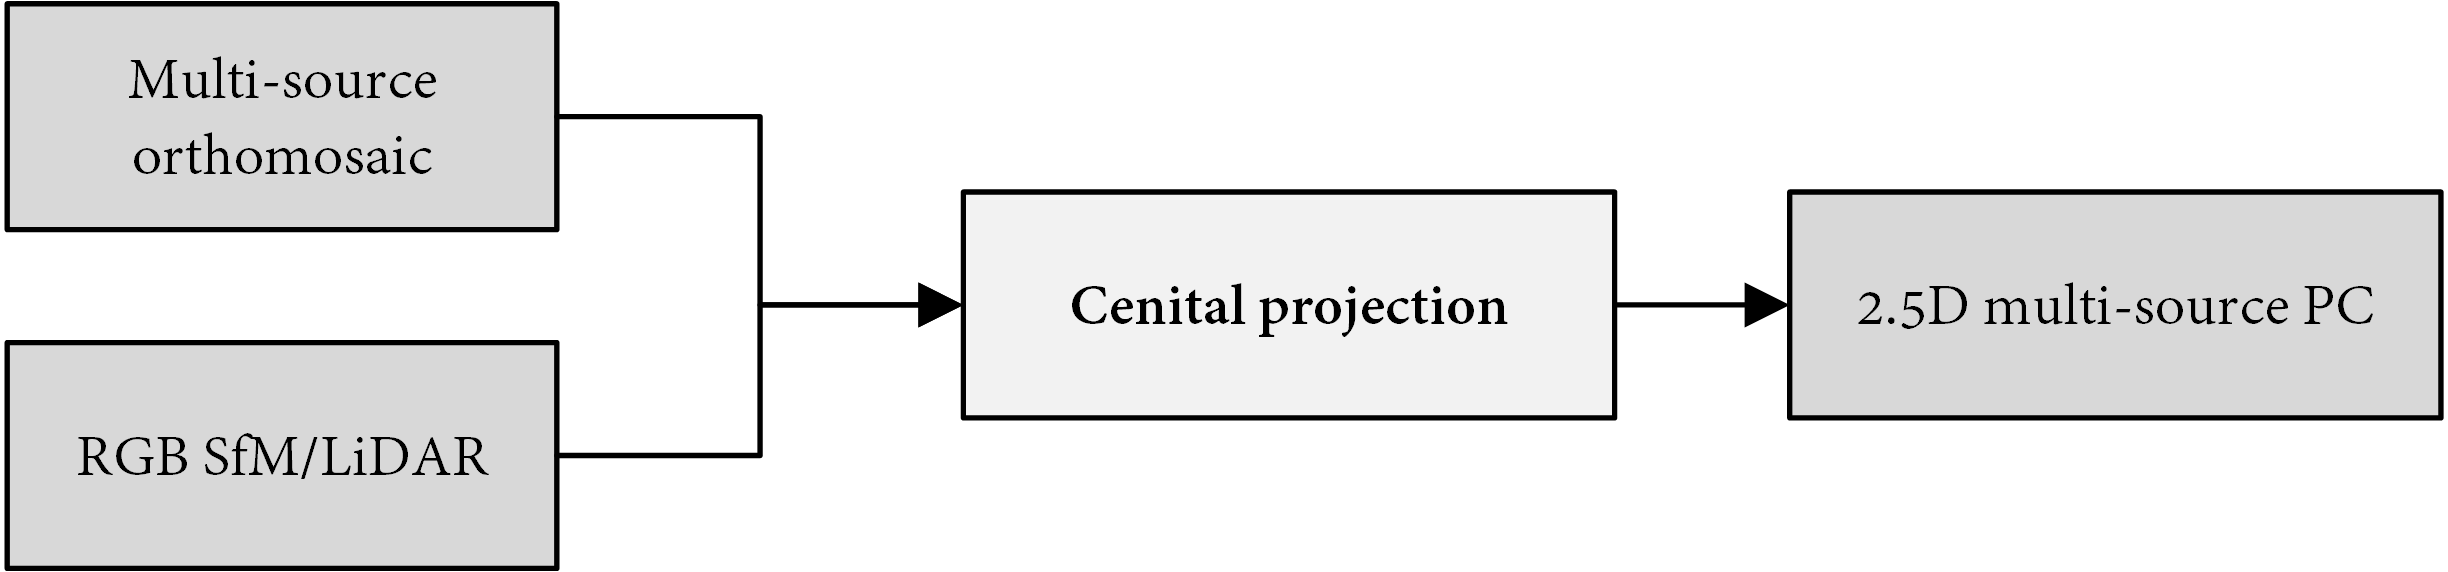
\includegraphics[width=\linewidth]{figs/context/fusion_02.png}
	\caption{2.5D point clouds are generated by projecting images from any data source into a baseline point cloud.}
    \label{fig:fusion_data_02}
\end{figure}

Finally, supervised procedures have also been proposed to match \acrshort{rgb} and thermal features. Huang et al. and Macher et al. \cite{huang_combining_2018, macher_combination_2019} used checkerboard images and relevant key points, such as building corners, to link features. Lafi et al. \cite{lafi_3d_2017} performed semi-automatic stitching of \acrshort{ir} images by marking relevant features, thus generating a panoramic image that was finally mapped to a 3D \acrshort{rgb} point cloud. However, semi-automatic registration is time-consuming and hard to apply over large datasets. Indeed, this procedure is more appropriate for datasets composed of a few images.

\subsection{Multispectral imaging}

The previous work focused on reconstructing 3D point clouds from multispectral imagery is coarsely split according to the use of satellite and \acrshort{uas} platforms. Traditionally, most of the previous work is based on satellite image mapping over 3D photogrammetric point clouds and \acrshort{lidar} models for monitoring the forest structure \cite{bolton_optimizing_2020, lechner_applications_2020}, multi-temporal observation of crops \cite{gadiraju_multimodal_2020, qadeer_spatio-temporal_2021} and semantic segmentation of urban and natural scenarios \cite{ballouch_toward_2022, saralioglu_semantic_2020}. State-of-the-art reconstruction methods from satellite data typically generate elevation data. \acrshort{dsm}s can be efficiently obtained with automatic image matching from multiple images acquired in the same orbit \cite{gui_automated_2021, qin_critical_2019}. Another promising field is the generation of super-resolution satellite images obtained with \acrshort{dl} \cite{gomez_experimental_2022, stucker_resdepth_2022}. Consequently, the cited advances and modern high-resolution satellite sensors enable recovering 3D surfaces from multi-view satellite panchromatic images \cite{han_state_2020, rothermel_photometric_2020}. The resulting 3D point clouds can be directly fused with multispectral bands of satellite imagery. 

Multispectral images acquired from \acrshort{uas} platforms have lower resolution than the majority of \acrshort{rgb} images, and yet, it is higher than the resolution provided by most \acrshort{ir} sensors. Therefore, 3D multispectral point clouds can be directly generated with photogrammetry \cite{liu_registration_2018, zainuddin_3d_2019, shen_estimation_2019, villacres_construction_2022, comba_unsupervised_2018}. Recently, Jurado et al. \cite{jurado_multispectral_2020} proposed a novel pipeline to generate dense multispectral point clouds by mapping images on dense \acrshort{rgb} point clouds. Firstly, a sparse \acrshort{nir} point cloud was reconstructed and aligned with the \acrshort{rgb} point cloud. The rest of the cameras were following projected and multispectral data was assigned to 3D \acrshort{rgb} points using \acrshort{knn}. Other approaches are based on multispectral data projection over 3D point clouds from \acrshort{rgbd} sensors embedded on aerial and terrestrial platforms. Clamens et al. \cite{clamens_real-time_2021} implemented a method based on feature-based and corner-based registration of \acrshort{rgbd} and multispectral images.

The integration of \acrshort{lidar} and multispectral sensors is another widely adopted approach. In recent years, the proliferation of lightweight \acrshort{lidar} sensors enables fusing data from a multispectral camera and \acrshort{lidar} sensor coupled to a \acrshort{uas}. Both sensors have usually the same \acrshort{gps} and \acrshort{imu} feed to avoid inconsistencies in the recorded time and space. Data fusion can be carried out by back-projecting data, i.e., rendering \acrshort{lidar} results from the optical camera’s perspective in order to correlate pixels and returns \cite{valbuena_integrating_2014}. Then, the pixel attributes are fetched and the \acrshort{lidar} returns are shaded. This projection is developed considering the optical sensor system (internal parameters) and the platform's position and bearing (external parameters). Sankey et al. \cite{sankey_quantifying_2021} proposed a novel methodology for \acrshort{uas}-based multispectral, hyperspectral and \acrshort{lidar} data fusion in shrub-encroached desert grassland. However, this study was based on a comparison between 2D multispectral and hyperspectral orthomosaics generated by Pix4Dmapper and SpectralView software, respectively. Gu et al. \cite{gu_uav-based_2020} integrated multispectral and \acrshort{lidar} sensors in a single system that simultaneously collected data. 

Photogrammetry can also help to generate orthomosaics of multispectral imagery, which can be later projected into \acrshort{rgb} point clouds \cite{comba_unsupervised_2018}. This procedure involves an orthogonal projection of multispectral orthomosaics to obtain 2.5D point clouds (see Figure \ref{fig:ortho_projection}). The main shortcomings of this approach are the geometric and radiometric inaccuracies obtained after computing an orthomosaic.

\subsection{Hyperspectral imaging}

The challenges of fusing \acrshort{hsi} and 3D models arise due to both data dimensionality and the required storage capacity. 3D reconstructions are easier to achieve with single-snapshot sensors since they can be generated using photogrammetry. However, push broom sensors pose several challenges due to the geometrical inaccuracies and the stitching of multiple swaths. This was already addressed in the fusion of 2D hyperspectral swaths, and it represents one of the first steps before fusing them with photogrammetric point clouds. 

The reconstruction of 3D hyperspectral point clouds has been previously achieved by fusing \acrshort{lidar} and \acrshort{hsi} \cite{lin_detection_2019, sankey_uav_2018}. Otherwise, it has been mainly addressed in close-range applications. For instance, Zia et al. \cite{zia_3d_2015} developed a method that applies \acrshort{sfm} to images from every collected wavelength and then, the wavelength-wise reconstructions were aligned. Kim et al. \cite{kim_3d_2012} described a system prototype composed of a laser sensor and a hyperspectral imager to characterize solid objects. Behmann et al. \cite{behmann_calibration_2015} proposed a method to generate 3D models from push broom sensors in close-range observations. This work used a polynomial transformation to describe the non-linear effects occurring in plant phenotyping, considering not only the linear model of the push broom sensors but also other distortion factors. The fusion of \acrshort{hsi} with models from laser scanners has also been addressed \cite{behmann_generation_2016}. Liu et al. \cite{liu_hyperspectral_2020} published an in-depth review of \acrshort{hsi} and 3D technologies for plant phenotyping by revising literature ranging from close-range applications to remote sensing. 

However, methodologies operating over measurements collected in the laboratory have a more controlled setup and stability in the sensor orientation. In contrast, these conditions are not guaranteed in outdoor scenarios with constantly changing conditions. For instance, the wind induces changes on the sensor and monitored scenes \cite{kalisperakis_leaf_2015}. Other works were capable of merging hyperspectral data in 3D models generated from standard \acrshort{rgb} cameras or laser scanning, thus enabling 3D geological modelling \cite{nieto_3d_2010} and 3D mapping of underwater environments \cite{ferrera_hyperspectral_2021}. 

Despite small-sized \acrshort{uas} enabling data acquisition with higher spatiotemporal resolution \cite{padua_uas_2017}, the integration of hyperspectral sensors is restricted due to payload capacity and flight autonomy \cite{bruning_approaches_2020}. These conditions harden their applicability to the monitoring of small-scale areas and research work. Even so, 3D hyperspectral modelling from \acrshort{uas} platforms is a recent technology that has become available to small-sized \acrshort{uas}s during the last decade \cite{nevalainen_individual_2017}. Some approaches use non-imager spectrometers in \acrshort{uas} platforms along with an \acrshort{rgb} sensor to accurately display the acquired spectral signatures over 3D information and orthomosaics acquired with \acrshort{rgb} data and photogrammetry \cite{garzonio_surface_2017}. For instance, Astor et al. \cite{astor_vegetable_2020} combined \acrshort{uas}-based \acrshort{rgb} data and ground-based \acrshort{hsi} for biomass estimation in different vegetable crops.

\acrshort{hsi} missions collect data by scanning and therefore, only a few perspectives of the area of interest are acquired in the flight direction, thus hardening the reconstruction of 3D scenarios. There is a void of methods accounting for this spatial heterogeneity to correctly merge hyperspectral data from push broom sensors into 3D models. With this approach, it would be possible to have a seamless data fusion integration that would lead to a very high spatial and spectral resolution. It can be expected that in the near future, \acrshort{uas}-based hyperspectral sensors will be capable of acquiring data in other parts of the \acrshort{em} spectrum, such as \acrshort{swir}, and even support on-board real-time processing \cite{horstrand_uav_2019, saari_visible_2017}.

\section{Simulation of Remote Sensing data}

Remote sensing imagers were conceived as mapping tools for generating products that help in the modelling and understanding of Earth's processes. However, the uprising combination of Remote sensing and \acrshort{ai} requires large datasets that enable trainable models to seek patterns in various scene perception tasks such as semantic segmentation, instance segmentation and classification applied over indoor and outdoor sceneries. Nonetheless, publicly available datasets may not suffix specific application requirements in terms of data density, attributes, kinds of scenes, recording platforms, etc. Amongst the most common examples of this is the advent of autonomous driving, which required large and variate annotated \acrshort{lidar} datasets to achieve safe systems capable of working under most conditions. Similarly, the semantic segmentation of \acrshort{lidar} has drawn the attention of both industry and academia. Multiple real-world \acrshort{lidar} datasets have been published over the last years, most of them focused on urban scenarios recorded with static or mobile platforms. Still, some of them are not labelled, do not include trajectories or \acrshort{gps}/\acrshort{imu} data, lack supplementary cameras, etc. \cite{cai_survey_2022}. 

The generation of synthetic \acrshort{lidar} data is among the most frequent computerized processes. However, the synthetic modelling of images has also been gaining interest \cite{yi_cycle_2023, ozkanoglu_infragan_2022}, especially for those spectral ranges which are not as widespread in publicly available datasets. For example, this is the case of infrared imagery, which is also influenced by the increasing demand for autonomous systems. Unlike visible cameras, infrared cameras do not rely on external light sources and therefore are appropriate for making autonomous systems understand their context even at night and in adverse daylight conditions. Among its applications, infrared may be required for reading traffic signals, wildlife and human detection and object tracking \cite{vollmer_infrared_2017}.  

\subsection{Motivation of synthetic \acrshort{lidar} simulation}

\acrshort{lidar} sensors are expensive imagers that require mobile or static platforms to generate a point cloud of the target scenario. To this end, one or multiple scans can be collected and joined by means of overlapping features. On the other hand, \acrshort{lidar} simulators are much more cost- and time-efficient once the emulation challenge has been resolved, which is neither trivial nor efficient to address. Simulating data avoids carrying out fieldwork to generate massive datasets and enables optimizing the planning of real \acrshort{lidar} scans \cite{mohan_robust_2019, li_3d_2022}. Instead of performing scans on real-world scenarios, simulations are performed over synthetic models that can be annotated with any \acrshort{lod}. Thus, these can feed the resulting point cloud with ground-truth data concerning a large number of attributes, from normal vectors to semantic annotations. 

There are multiple applications of \acrshort{lidar} simulations, along with their corresponding research niches. From a hardware perspective, some simulators are focused on the design, validation and calibration of \acrshort{lidar} sensors \cite{lee_validation_2020}. Their objective is to detect and reduce errors in the scanning, both systematic and random. There are also simulators focused on the optimization of scanning processes \cite{iqbal_simulation_2020, westling_simtreels_2020}, such as the integration of \acrshort{lidar} data into enhanced and synthetic vision systems \cite{peinecke_lidar_2008}. From a software perspective, one of the most popular research topics is autonomous driving \cite{fang_augmented_2020, li_deep_2020} and navigation \cite{manivasagam_lidarsim_2020}. Most of these methods, especially those based on \acrshort{dl}, benefit significantly from synthetic data. 

Beyond generic research purposes, including teaching and learning, there are systems aimed at the custom configuration of the simulated sensors, including their mounting platform and setup. These simulators typically allow the user to fine-tune all the parameters needed for a physically-based simulation of the laser beams and the interaction with the virtual environment, where photon mapping, Monte Carlo simulation, and full \acrshort{lidar} waveform generation are their core foundations \cite{yun_simulation_2019, chen_ole_2020, zohdi_rapid_2020}. These frameworks can simulate multiple scattering of the laser beams, taking into account their propagation through wind-driven rough air-water interface \cite{chen_ole_2020}, or vegetation \cite{yun_simulation_2019, westling_simtreels_2020}. There also exist commercial and open-source software such as LGSVL (LG) \cite{lg_electronics_rd_lab_lgsvl_2021}, Simcenter (Siemens Software) \cite{siemens_simcenter_2021}, and CARLA \cite{dosovitskiy_carla_2017} for generating autonomous driving datasets.

\subsection{Public \acrshort{lidar} datasets}

The vast majority of \acrshort{lidar} datasets focus on autonomous driving and perception tasks such as classification, semantic segmentation, instance segmentation and tracking of mobile objects \cite{chen_automatic_2022}, using geometrical \cite{behley_towards_2021} and intensity information \cite{tan_toronto-3d_2020}. Most of them record metropolitan environments from a mobile vehicle coupled with a \acrshort{lidar}, along with visible and infrared cameras in a few case studies \cite{choi_kaist_2018}. On the other hand, aerial \acrshort{lidar} datasets covering large portions of the Earth's surface are frequently published by governmental institutions at land inventorying portals. Since these are intended to cover large areas, they are acquired from mid-altitude platforms with a density of a few points per squared meter (up to two points according to the United States Geological Survey \cite{us_geological_survey_lidar_2012} and 0.5 points for the Spanish National Plan of Land Observation \cite{instituto_geografico_de_informacion_geografica_pnoa_nodate}). More recently, despite not being frequent, large and denser aerial \acrshort{lidar} datasets have also been published \cite{varney_dales_2020}. 
\begin{marginfigure}[.0cm]
	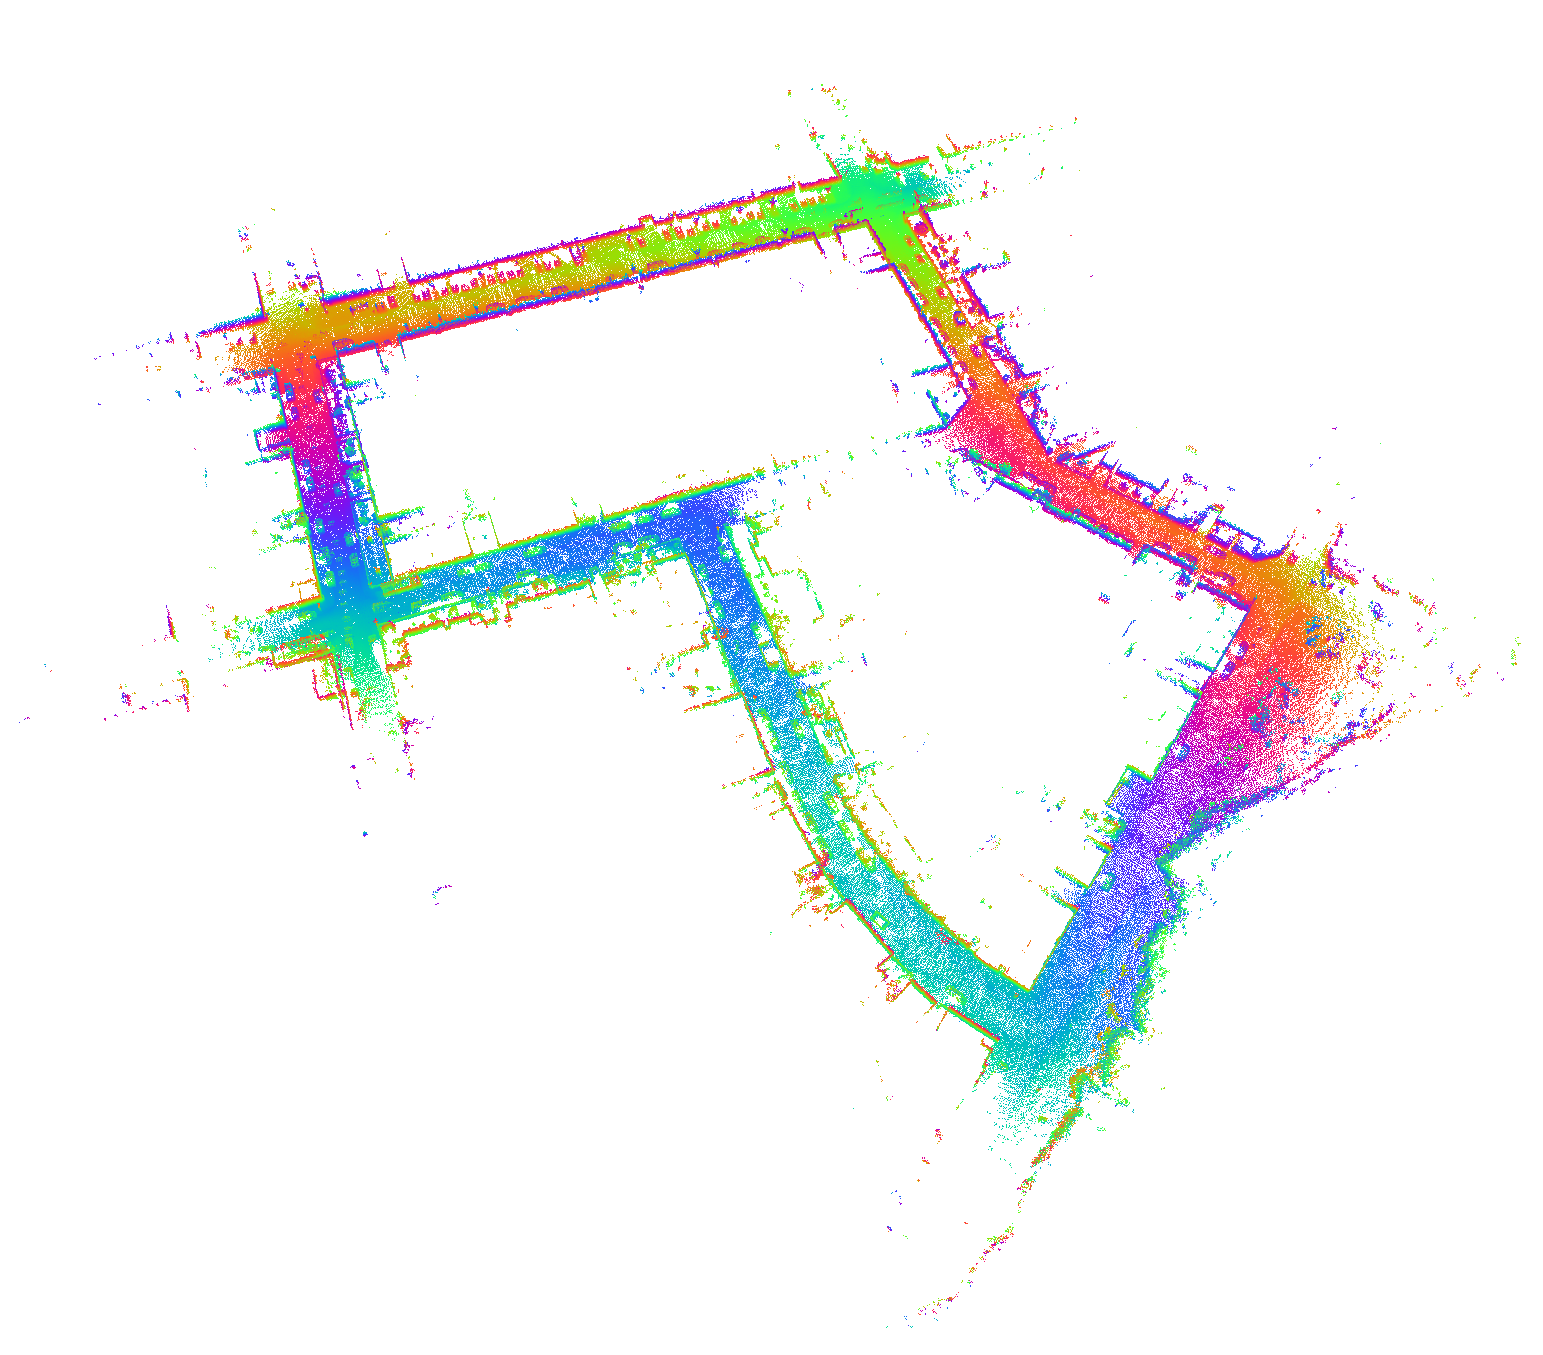
\includegraphics{figs/context/kitty_scan.png}
	\caption{Example of a metropolitan \acrshort{lidar} point cloud in the SemanticKITTI dataset \cite{behley_towards_2021}, composed of a sequence of scans recorded from a vehicle coupled with a Velodyne \acrshort{lidar}.}
	\label{fig:kitty_scan}
\end{marginfigure}

Both kinds of datasets, terrestrial and aerial, are required to be annotated to be applied to \acrshort{dl}. Previously revised datasets are recorded by real sensors, and therefore, their classification must be performed manually \cite{behley_towards_2021, pan_semanticposs_2020, tan_toronto-3d_2020} or automatized with networks trained with very limited data \cite{wu_squeezesegv2_2019}. Manual labelling induces errors, but another shortcoming is the lack of detail. For example, these are some real datasets and the number of different semantic labels: SemanticKITTI (25) \cite{behley_towards_2021}, nuScenes (23) \cite{caesar_nuscenes_2020}, SemanticPOSS (14) \cite{pan_semanticposs_2020}, Toronto-3D (8) \cite{tan_toronto-3d_2020} and Semantic3D (8) \cite{hackel_semantic3d_2017}. More recently, \acrshort{lidar} datasets have been released together with video and audio data \cite{piadyk_streetaware_2023} (see Figure \ref{fig:lidar_audio_video}). A more complete compilation of open-source real \acrshort{lidar} datasets can be found in \cite{cai_survey_2022}. 

\begin{figure}[ht]
	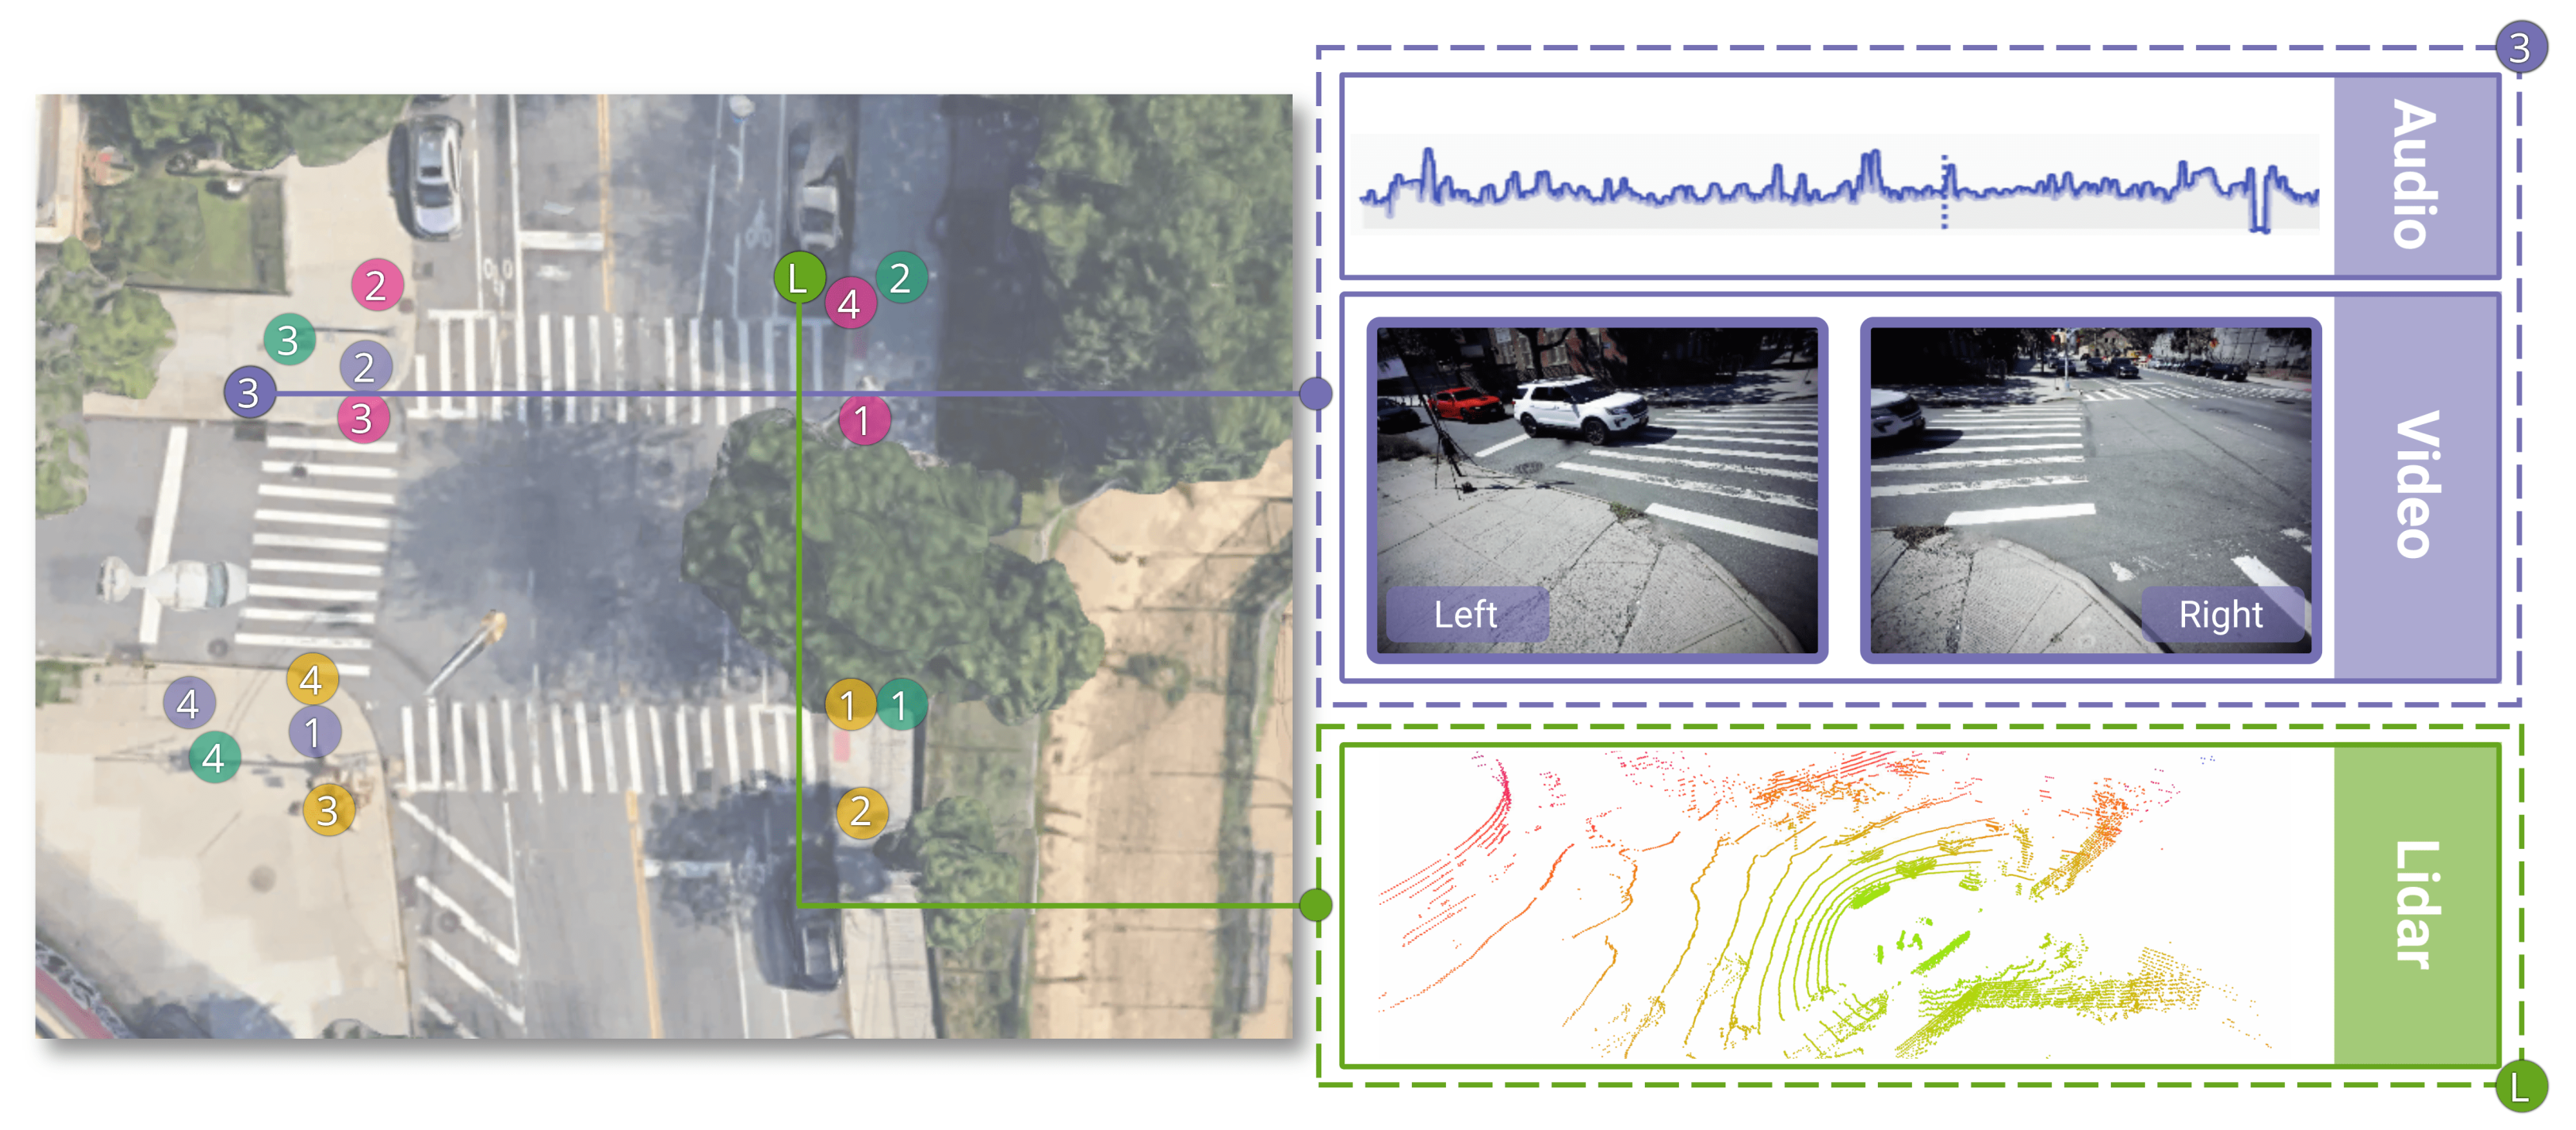
\includegraphics[width=\linewidth]{figs/context/lidar_dataset_audio_video.png}
	\caption{Overview of the data collection proposed by Piadyk et al. \cite{piadyk_streetaware_2023}, where \acrshort{lidar} is captured along with audio and video feed. }
    \label{fig:lidar_audio_video}
\end{figure}

\subsection{\acrshort{lidar} simulation}

The early \acrshort{lidar} simulators produced graphically feasible \acrshort{lidar} point clouds \cite{gschwandtner_blensor_2011} by emulating the sensor's \acrshort{fov}, occlusion and beam divergence. \acrshort{lidar} returns can be solved with ray-casting \cite{ahn_real-time_2020, zhao_method_2021, bechtold_helios_2016} in annotated environments. Remark that ray-casting implies solving impacts of laser beams in the followed path, frequently ranging from one to five returns, whereas ray-tracing refers to emulating light interaction among surrounding surfaces. The latter represents a physically-based simulation that requires an enormous computation effort and therefore is not yet practical \cite{ahn_real-time_2020}. In recent years, \acrshort{lidar} simulators have addressed the realistic simulation of geometry returns, the impact of surface properties as well as other environmental conditions. 

Some of the aspects of what is expected from physically-based results have been simulated by including a wide number of errors and limitations. First, Xhao et al. \cite{zhao_method_2021} modelled atmospheric effects such as rain, snow and fog by including signal attenuation and noise. Haider et al. \cite{haider_development_2022} have recently modelled the signal processing of \acrshort{lidar} as well as scan patterns to emulate optical losses and defects. Among the cited features, signal attenuation \cite{dosovitskiy_carla_2017, bechtold_helios_2016, hanke_generation_2017}, beam divergence \cite{zhao_method_2021, bechtold_helios_2016, hanke_generation_2017, haider_development_2022} and drop-off in intensity \cite{ahn_real-time_2020} are frequent in the literature. Very few address multiple returns \cite{winiwarter_virtual_2022} despite simulating beam divergence. Other not-that-frequent errors are mirror reflection \cite{ullrich_advances_2019}, motion distortion \cite{chen_analysis_2022}, non-uniform density and distortion of point attributes (colour, intensity, etc.), either as a result of an inappropriate setup \cite{dimitrov_segmentation_2015}, or systematic and random errors \cite{isheil_systematic_2011, fan_error_2015, pandzic_error_2017}. Random errors depend on aspects like the signal-to-noise ratio of the received signal, the accuracy of the electronics (including again the \acrshort{imu} and the \acrshort{gps}), the divergence of the laser beams (jittering) and their wavelength, as well as the reflectivity of the objects. Instead of physically emulating these features, previous work has deviated ideal synthetic \acrshort{lidar} point clouds with \acrshort{dl} \cite{manivasagam_lidarsim_2020, xiao_synlidar_2021, guillard_learning_2022}. The leveraging of real \acrshort{lidar} and synthetic point clouds has also been investigated by mixing scanned urban scenarios and synthetic objects \cite{manivasagam_lidarsim_2020}. Nonetheless, annotation and ground-truth shortcoming remains when leveraging both kinds of data.

\begin{marginfigure}[.0cm]
	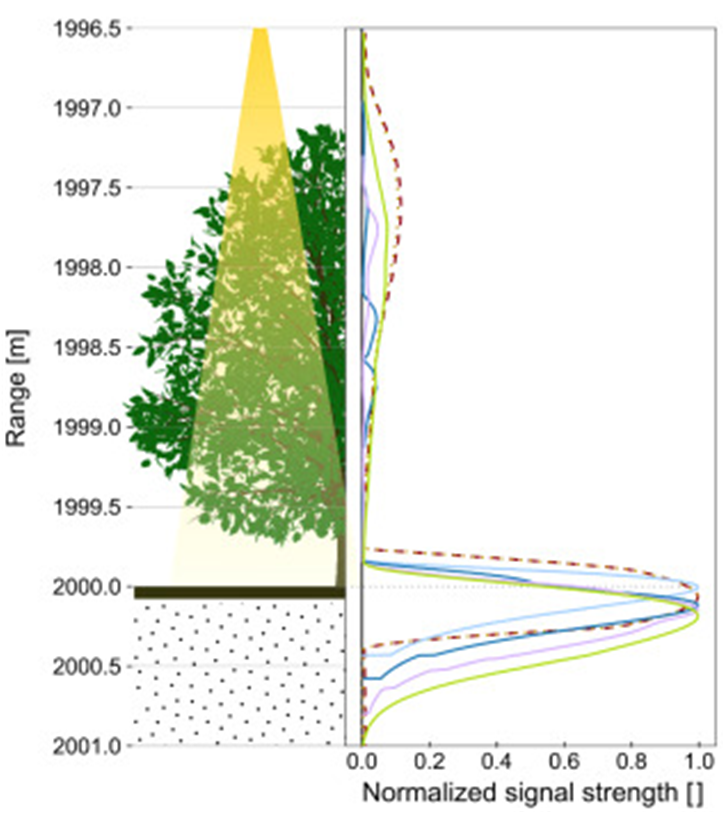
\includegraphics{figs/context/waveform_lidar.png}
	\caption{Simulation of a full-waveform \acrshort{lidar} traversing a tree \cite{winiwarter_virtual_2022}.}
	\label{fig:full_waveform_lidar}
\end{marginfigure}
Most of the revised simulators are focused on Terrestrial Laser Scanning (\acrshort{tls}), while Airborne Laser Scanning (\acrshort{als}) has barely been addressed \cite{winiwarter_virtual_2022}. Westling et al. \cite{westling_simtreels_2020} included \acrshort{als} as an unrealistic extension of \acrshort{tls}. Bechtold and Höfle \cite{bechtold_helios_2016} simulated \acrshort{als} with different scanning geometries (Figure \ref{fig:scan_geometries_lidar}), which is one of the main challenges of \acrshort{als}. More recently, Winiwater et al. \cite{winiwarter_virtual_2022} extended the work of Bechtold and Höfle to incorporate full-waveform \acrshort{lidar} (Figure \ref{fig:full_waveform_lidar}. Rather than capturing discrete returns, this kind of sensor returns the intensity recorded over a path. For instance, it helps to measure the amount of vegetation at different altitudes for forest inventory. One of the main inconveniences of this solution, published under the name of HELIOS++, is that input environments are simplified by means of voxels and therefore lose part of the scene details.

\begin{figure}[ht]
	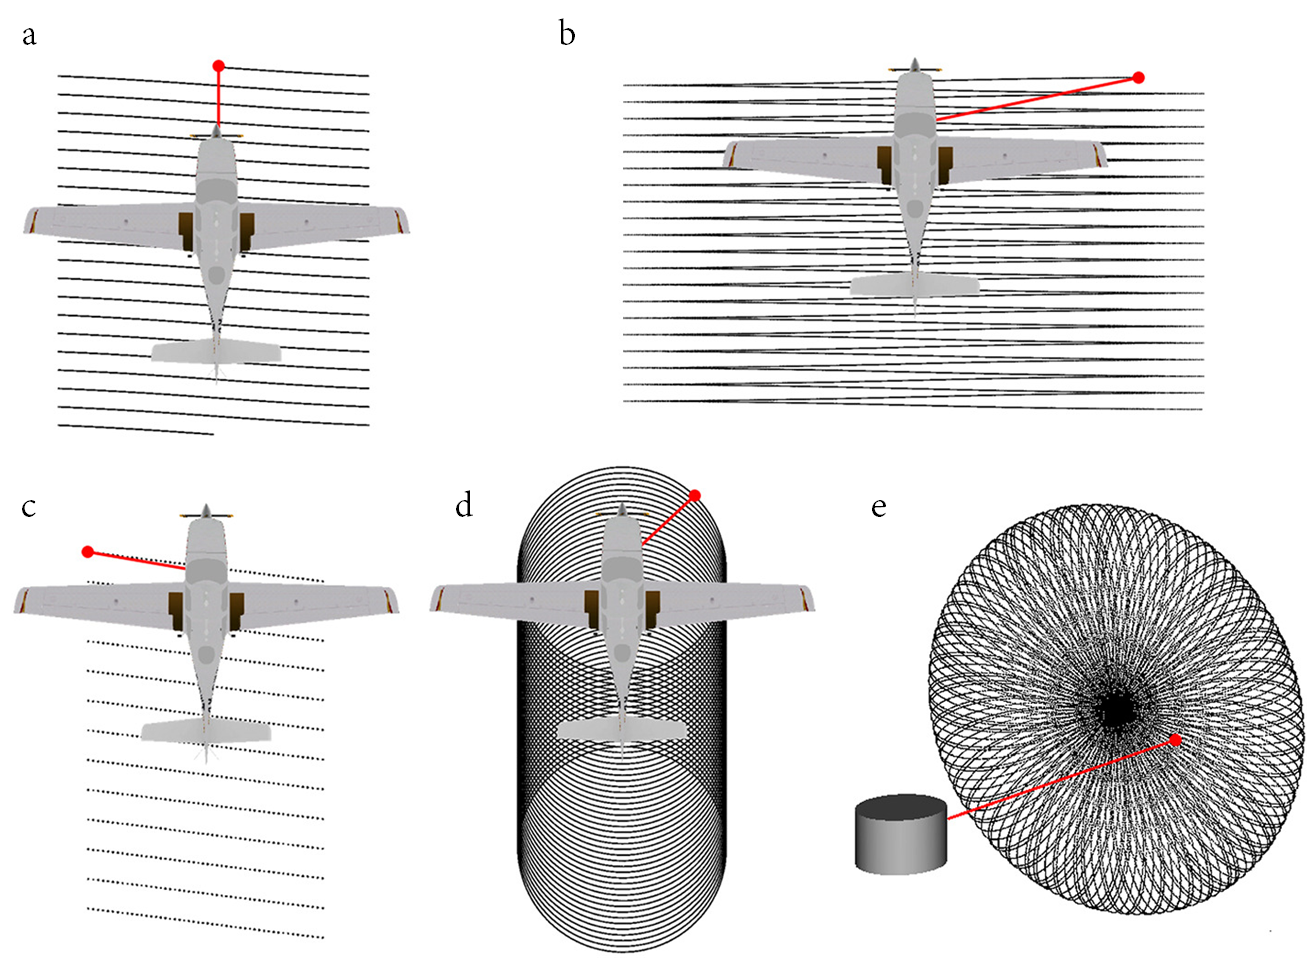
\includegraphics[width=\linewidth]{figs/context/scan_geometries_lidar.png}
	\caption{Overview of different scanning geometries from the HELIOS++ simulator: a) rotating mirror, b) oscillating mirror, c) fibre-optic line scanner, d) slanted rotating mirror (Palmer scanner), and e) Risley prisms (i.e., Livox scanner). }
    \label{fig:scan_geometries_lidar}
\end{figure}

On the other hand, the modelling of materials typically estimates the reflectance using phenomenological \acrshort{brdf}s such as Oren-Nayar, Lambertian and Blinn-Phong \cite{chen_analysis_2022}, regardless of the sensor wavelength \cite{chen_analysis_2022, gschwandtner_blensor_2011, zohdi_rapid_2020}. Other studies use diffuse, specular and transmissive properties acquired from commercial frameworks, such as CarMaker \cite{haider_development_2022}. Intensity has also been simulated using \acrshort{dl} with \acrshort{lidar} data represented as images instead of points \cite{vacek_learning_2022, xiao_synlidar_2021}. However, these networks are constrained to the variety of materials and lighting conditions in the training datasets. 

\subsection{Time efficiency}

Most studies do not evaluate the efficiency of the proposed solution, and \acrshort{dl} networks are constrained to the response time of the network. To the best of our knowledge, only Peinecke et al. \cite{peinecke_lidar_2008} have considered a \acrshort{gpu}-based simulation in \acrshort{opengl}. Also, the efficient semantic labelling and generation of synthetic environments have been poorly addressed, including the annotation of virtual scenes composed of \acrshort{cad} models. Another key factor is the precision of the synthetic scans: previous work has simulated \acrshort{lidar} scans using depth buffers \cite{su_simulation_2019, fang_augmented_2020, manivasagam_lidarsim_2020} with a limited resolution, frequently $2^8$ unless the target texture is composed of floating-point values. 

\section{Optimization of LiDAR scans in indoor environments}

\subsection{Motivation} 

\acrshort{lidar} is widespread in the construction industry for the tracking of building progress by enabling the acquisition of the environment geometry in a precise and highly detailed way. Instead of polygonal meshes, a discretized representation of buildings is given by point clouds. To achieve this goal, \acrshort{tls} is increasingly being used to collect large sets of building data \cite{pandzic_error_2017}. This technology can be applied to a wide range of applications, including building inspections \cite{shariq_revolutionising_2020}, monitoring of natural environments (landform dynamics \cite{guisado-pintado_3d_2019}, ecological resilience \cite{mitasova_geospatial_2010}, etc.), autonomous driving \cite{kuutti_survey_2021} or preservation of cultural heritage \cite{banfi_integration_2019, ham_phased_2020, andriasyan_point_2020}, among others. Besides terrestrial scanners, \acrshort{lidar} technology presents multiple variants according to their capabilities (range, spatial resolution and covering, etc.) and the platform from which they are operated (\acrshort{als}, \acrshort{tls}, \acrshort{mls}, \acrshort{bmmls}, etc.) \cite{poux_smart_2019, warchol_concept_2019}. 

Some of the main challenges of \acrshort{tls} in the surveying of 3D facilities are the occlusion and range limitations \cite{soudarissanane_optimizing_2012}. Consequently, appropriate planning of \acrshort{tls} scans is necessary in order to 1) minimize the number of different acquisition points, 2) generate a uniformly dense point cloud, and 3) reduce the occlusion from scene objects. These three objectives are equally influenced by the configuration and placement of the scanner. On the other hand, periodic scanning and monitoring of buildings are especially relevant for digitized representations, such as the widely known Building Information Modelling (\acrshort{bim}) \cite{macher_point_2017}. They encode characteristics of a building, including 3D design drawings, materials, costs and safety specifications \cite{patraucean_state_2015}, and provide an interface for the management of 4D applications. Together with \acrshort{tls}, it allows the monitoring of continuously evolving buildings to preserve cultural heritage, track its current state and maintain repair records \cite{rocha_scan--bim_2020, andriasyan_point_2020, moyano_bringing_2020, ham_phased_2020}. However, the monitoring of buildings over time is time-consuming, especially in dynamic environments. Also, \acrshort{tls} surveys generate multiple point clouds that need to be fused either by placing target marks \cite{gollob_comparison_2020} or by estimating the rigid transformation that minimizes the distance among overlapping point clouds. In order to speed up this acquisition task, the development of tools for the planning of \acrshort{tls} surveys plays a key role.

\subsection{Planning for Scanning}

The Planning for Scanning (\acrshort{p4s}) has previously been addressed using a wide range of environments and techniques. If the number of target locations is known, then the selection of an optimum set is also known as the NP-complete set-coverage problem \cite{li_probability_2021, mohamadi_efficient_2021, roostapour_pareto_2022}. Previous research can be categorized according to the input environment: model-based or non-model-based (discovered as being explored). The latter is mainly applied to robotic applications whose environment is unknown \cite{potthast_probabilistic_2014}. Otherwise, input scenarios are either defined as 2D or 3D models, with 2D representations being cross-sections of buildings \cite{giorgini_sensor-based_2019}. Solutions for 2D inputs present lower computational complexity and are frequently solved following an iterative selection of viewpoints (Next Best View; \acrshort{nbv}) or heuristic algorithms \cite{aryan_planning_2021}. The main drawback of these algorithms is that they do not consider the details underneath complex buildings. Instead, they are focused on 2D sketches composed of wall edges. 3D-based approaches are far more complex and guided by metrics that allow filtering and ordering spatial locations, as in Figure \ref{fig:planning_for_scanning_room}. Despite this, the exploration of 3D buildings is also approached with heuristics and \acrshort{nbv}. However, the high latency frequently leads to simplifications of the environment using voxelizations \cite{wakisaka_optimal_2019, rougeron_optimal_2022}, axis-aligned bounding boxes (\acrshort{aabb}) and object-oriented bounding boxes (\acrshort{oobb}) \cite{li_3d_2022}. A similar work to ours was published at the same time, also partly implemented in \acrshort{gpu} \cite{rougeron_optimal_2022}. However, the environment was voxelized and the number of optical locations was set by users, instead of being part of the optimization. On the other hand, Chen et al. \cite{chen_3d_2022} solved the \acrshort{p4s} optimization over 3D scanned façades using a Greedy algorithm. The weight of each location was estimated from a \acrshort{lidar} simulation. Finally, 2.5D models, such as \acrshort{dsm}s, have also been investigated in a similar way to 2D environments \cite{starek_viewshed_2020}.

\begin{figure}[ht]
	\includegraphics[width=\linewidth]{figs/context/planning_for_scanning.png}
	\caption{Example of 3D model for experimentation of \acrshort{p4s}. The main scene has another inner room which some gaps which serve to stress the planning for scanning algorithm. It helps to show how algorithms perform in terms of \acrshort{lod}, \acrshort{loa} and \acrshort{loc}.}
    \label{fig:planning_for_scanning_room}
\end{figure}

\subsection{Metaheuristics}

Heuristics are the most frequent solver in \acrshort{p4s}. Although they do not provide optimal solutions, they are proven good enough to cover environments with minimum scanning locations. Among heuristics, the Greedy algorithm has been extensively investigated \cite{zhang_rapid_2016, giorgini_sensor-based_2019, heidari_mozaffar_optimal_2016}, followed by Simulated Annealing (\acrshort{sa}) \cite{chen_indoor_2018}, Genetic Algorithms (\acrshort{ga}) \cite{jia_comparison_2017}, Particle Swarm Optimization \cite{jia_comparison_2017} and Integer Programming \cite{wakisaka_optimal_2019}. Greedy algorithms are based on the iterative selection of locations, according to an objective function. Other Greedy variations weight the locations using a visibility score \cite{jia_comparison_2017}, while others are followed by \acrshort{sa} \cite{latimer_sensor_2004}, or optimized with Divide and Conquer (\acrshort{d&c}) \cite{zhang_rapid_2016}. Instead of providing an automatic pipeline, \cite{ahn_interactive_2016} proposed an interactive semi-automatic system.

\begin{figure}[ht]
	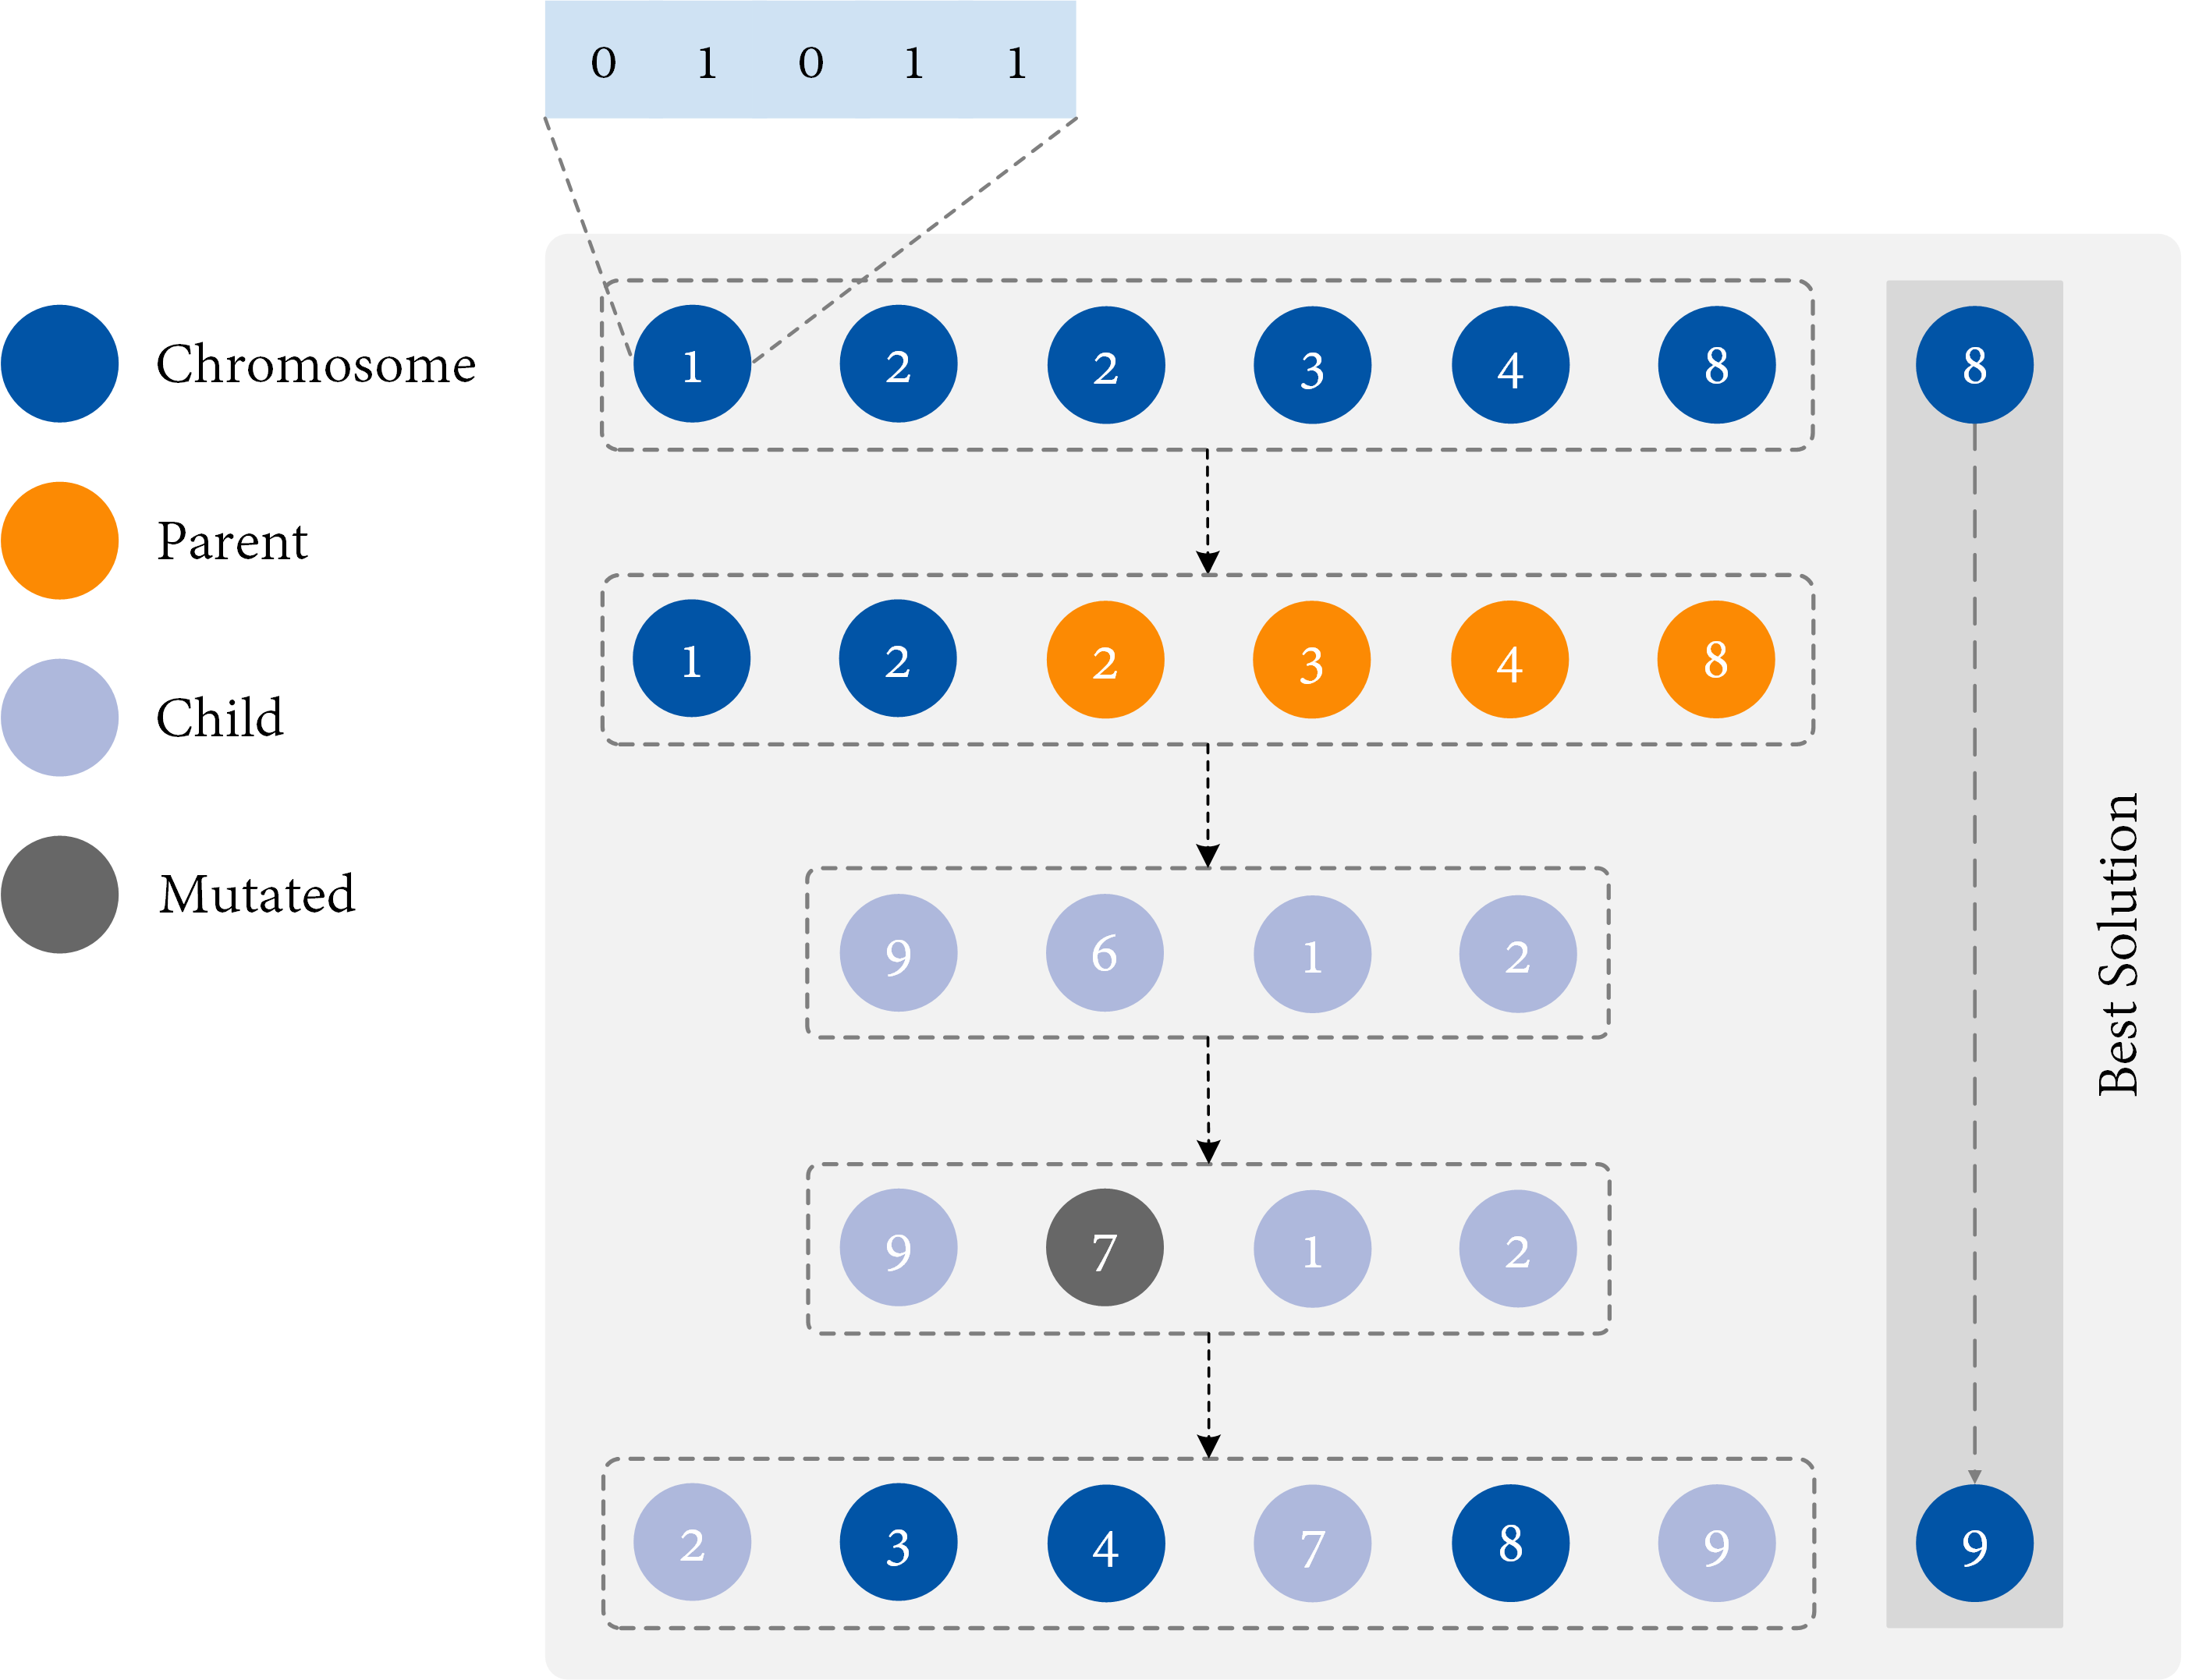
\includegraphics[width=\linewidth]{figs/context/genetic_algorithm.png}
	\caption{Overview of the iterative process and data encoding in a Genetic Algorithm (\acrshort{ga}). }
    \label{fig:genetic_algorithm}
\end{figure}

Heuristic solvers are guided by objective functions measuring the quality of achieved solutions. To evaluate this, four metrics are frequently used in previous work \cite{li_3d_2022, aryan_planning_2021}: Level of Detail (\acrshort{lod}), Level of Accuracy (\acrshort{loa}), Level of Overlap (\acrshort{loo}) and Level of Coverage (\acrshort{loc}). \acrshort{lod} refers to the point cloud resolution, \acrshort{loa} measures the quality of \acrshort{lidar} returns, as higher distances and angles deteriorate the quality of the measurements \cite{ aryan_planning_2021}, \acrshort{loo} refers to the overlapping area among point clouds so that \acrshort{tls} scans can be joined with rigid transformation estimations (e.g., \acrshort{icp}), and \acrshort{loc} refers to the number of polygons reached by scans. Thus, the optimization is very influenced by the \acrshort{lidar} range and incidence angles. 

\begin{marginfigure}[3.0cm]
	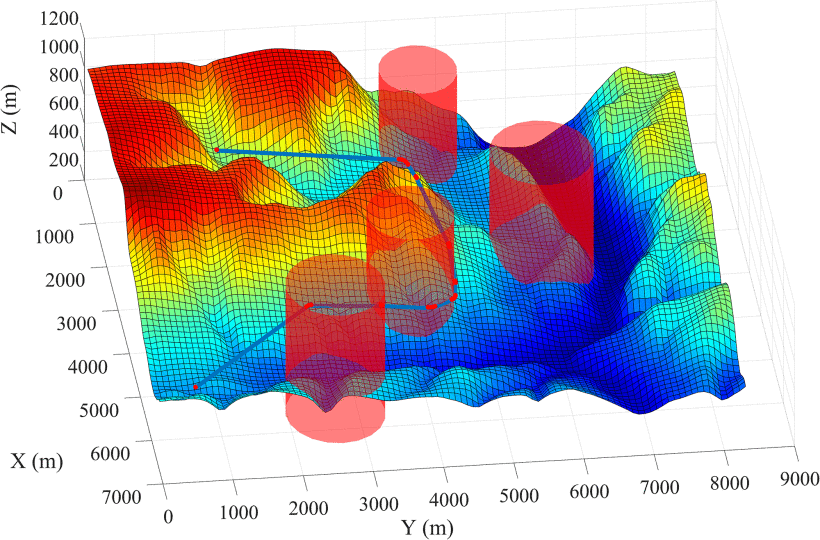
\includegraphics{figs/context/uav_path_planning.png}
	\caption{Path planning of a fixed-wing military \acrshort{uas} with the objective of minimizing flight altitude and fuel consumption.}
	\label{fig:path_planning_uav}
\end{marginfigure}
Research on heuristics in 3D is also frequent in the literature, though they are mostly linked to path planning \cite{pehlivanoglu_enhanced_2021, roberge_parallel_2021} (see Figure \ref{fig:path_planning_uav}) and the selection of subsets \cite{pehlivanoglu_enhanced_2021}. However, the number of scans needed to meet the required quality is unknown in a non-finite 3D space. The set of possible solutions can be narrowed either by selecting random locations \cite{chen_indoor_2018} or sampling the environment as a 2D grid \cite{starek_viewshed_2020, giorgini_sensor-based_2019, jia_comparison_2017}. For uniform subdivisions, the level of detail of the tessellation is a key factor with regard to response time. Coarse subdivisions present lower latency, though they are prone to yield far from optimal solutions. Starek et al. \cite{starek_viewshed_2020} enhanced initial locations by applying minor translations while assessing their quality through an objective function, whereas Soudarissanane and Lindenbergh \cite{soudarissanane_optimizing_2012} improved the sampling by increasing the grid subdivisions, at the expense of higher response time. For 3D locations, Starek et al. \cite{starek_viewshed_2020} described a \acrshort{sa} procedure to translate uniformly sampled points into surrounding locations that improve the covering metric. Kim et al. \cite{kim_placement_2020} tried to find the optimal \acrshort{lidar} position over an autonomous vehicle using Genetic Algorithms (\acrshort{ga}). For that purpose, the specifications of commercial \acrshort{lidar}s were used to compute the occupancy grid, defined as a discretized $360^\circ$ map represented by several views acquiring the coverage region and dead zones. Beyond theoretical/simulation approaches, multiple studies focus on evaluating the set-up of several sensors, concerning height, angles and location in autonomous driving \cite{pereira_self_2016, veronese_accurate_2018}. 

Once locations are locally optimized, they are processed as a classic set-coverage problem \cite{soudarissanane_optimizing_2012}. Recent research has solved this with \acrshort{ga}, using different operators and configurations \cite{wang_solving_2018, roostapour_pareto_2022, mohamadi_efficient_2021}. Local searches \cite{li_probability_2021} and other nature-inspired heuristics \cite{islambouli_optimized_2019} are also reviewed. Despite heuristics being allowed to solve hard problems with optimal or nearly optimal solutions, these are not efficient in most cases. Previous studies regarding \acrshort{p4s} required hours, even days, to determine the optimal scanning configuration in 3D environments. Even 2D-based approaches are time-consuming \cite{giorgini_sensor-based_2019} if they are implemented in a sequential manner. Thus, multi-core and \acrshort{gpu}-based approaches offer a huge improvement in the response time, reducing it to a few seconds or minutes \cite{giorgini_sensor-based_2019, wang_solving_2018, roberge_parallel_2021}. 

\section{Analysis of Remote sensing data}

\subsection{Vineyard phenotyping}

\subsubsection{Motivation}

Understanding vegetation development is a crucial aspect of crop management that impacts the effectiveness and productivity of agricultural efforts. Precision Agriculture (\acrshort{pa}) involves observing agricultural variables that affect crop production, which enables accounting for spatial and temporal variations, resulting in enhanced crop performance, reduced costs, and improved sustainability. Additionally, it provides a forecasting tool to accurately supply crop needs, such as water and nutrients. If applied to vines, the concept becomes Precision Viticulture (\acrshort{pv}), with a wide variety of applications, ranging from the detection of biomass \cite{di_gennaro_evaluation_2020}, water content \cite{santesteban_high-resolution_2017, gutierrez_assessing_2021} and other compounds \cite{peng_prediction_2022}, to vigour estimation \cite{bramley_12_2010, campos_development_2019}, detection of plant diseases, pest surveillance \cite{mendes_vineinspector_2022}, analysis of grape maturity \cite{soubry_monitoring_2017} or yield estimation \cite{hassanzadeh_broadacre_2021}. They are either focused on grape clusters, leaves, stems or vineyard support \cite{singh_bibliometric_2022}. 

\begin{figure}[ht]
	\includegraphics[width=\linewidth]{figs/context/vineyard_plot.jpg}
	\caption{Wide angle view of a vineyard plot.}
    \label{fig:vineyard_plot_sample}
\end{figure}

The characterization of vineyard plots using \acrshort{uas}s is particularly challenging due to their variability, regarding the tree structure, inter-row spacing and surrounding elements (bare soil, shadowed areas, grassing, etc.), as depicted in Figure \ref{fig:vineyard_plot_sample}. Therefore, high-detailed images are relevant for discriminating vegetation, soil and weeds, which have been previously shown to affect grape estimations \cite{ammoniaci_state_2021, sassu_advances_2021}. Consequently, a significant effort of previous studies is oriented toward the segmentation of the canopy \cite{padua_vineyard_2022}. In this regard, \acrshort{uas}s help to support decision-making systems by gathering precise information that enables the estimation of biophysical and performance-related features \cite{bramley_12_2010}.

\subsubsection{Traditional hyperspectral classification}

\acrshort{dl} methods have recently become the preferred approach for classifying hyperspectral imagery. However, earlier techniques relied on comparing the acquired data to reference reflectance shapes that were ideally measured in a laboratory. The primary objective of these methods was to measure the similarity between labelled and unlabelled spectral shapes. Spectral libraries, containing data measured from a spectrometer, were used for this purpose. For instance, there exist spectral libraries for minerals, trees, and daily surfaces \cite{kokaly_usgs_2017, dutta_characterizing_2017, matusik_data-driven_2003}. These methods varied from the widely used Euclidean distance to more sophisticated techniques such as Spectral Angle Matching (\acrshort{sam}), Cross-Correlogram Spectral Matching (\acrshort{ccsm}), and probabilistic approaches like Spectral Information Divergence (\acrshort{sid}) \cite{pu_hyperspectral_2017}. Among these techniques, \acrshort{sid} and \acrshort{ccsm} have been found to perform better in mineral classification from Aviris data. Similarly, van der Meer \cite{van_der_meer_effectiveness_2006} proved that \acrshort{sam} introduced much more confusion than \acrshort{sid} and Spectral Correlation Matching (\acrshort{scm}) in a case study of mineral classification. \acrshort{sam} has the advantage of being invariant to different scales, making it useful for heterogeneous acquisition devices and conditions. Other techniques derived from \acrshort{sam} include Spectral Correlation Angle (\acrshort{sca}), based on the Pearson correlation coefficient, and Spectral Gradient Angle (\acrshort{sga}) \cite{ren_novel_2022}. In addition to similarity, angular and probabilistic measures, the literature describes other error- and colourimetric-based methods. The former group includes the widely used Mean Square Error (\acrshort{mse}), Root Mean Square Error (\acrshort{rmse}), Mean Relative Absolute Error (\acrshort{mrae}), Back-Projection MRAE (\acrshort{bpmrae}) and the Peak Signal-to-Noise Ratio (\acrshort{psnr}) \cite{agarla_analysis_2021}. More recently, Kumar et al. \cite{kumar_new_2021} introduced three new metrics (Dice Spectral Similarity Coefficient (\acrshort{dssc}), Kumar–Johnson Spectral Similarity Coefficient (\acrshort{kjssc}), and a hybrid of the previous, KJDSSC$_{\textit{tan}}$) that outperformed traditional techniques on mineral and vegetation classification.

Colourimetric measures involve measuring distance in various colour spaces, such as pro-Lab. Agarla et al. \cite{agarla_analysis_2021} have compared all these techniques to assess their correlation and determine the most significant ones. Additionally, spectral derivatives, which are finitely approximated considering the previous spectral sample and wavelength distance, are used to remove or compress illumination variations resulting from acquisition conditions \cite{fernandes_grapevine_2019, pu_hyperspectral_2017}. These techniques are still applied when the reflectance profile of different materials exhibits notable variations. Furthermore, semi-automatic classification methods have been reviewed for situations where classification involves only a few labels. For instance, Ahmed et al. \cite{ahmed_applied_2021} used \acrshort{pca} to extract features from multispectral imagery and proposed a vegetation index to label different trees. Pádua et al. \cite{padua_monitoring_2020} described similar work on classifying chestnuts with phytosanitary problems using two new indices: Ex\acrshort{nir} and ExRE, where Ex refers to Excess and Re to Red. However, these techniques are not suitable for differentiating a significant number of vineyard varieties since they all exhibit similar shapes. We refer the reader to \cite{shanmugam_spectral_2014} for an in-depth revision of spectral matching and attributes conditioning the construction of spectral libraries.

\subsubsection{Hyperspectral transformation and feature extraction}

In this section, the transformations that facilitate classification using traditional methods are discussed. Due to the extensive coverage of land by satellite imagery, it is uncommon for hyperspectral pixels to depict the spectral signature of a single material. Therefore, there is a prevalent topic in the hyperspectral literature, which involves breaking down the acquired Earth's surfaces by analyzing the hyperspectral images. The problem is illustrated with $\rho = \textit{MF} + \epsilon$, where $M$ is the spectral signature of different materials, $F$ is the weight, $\epsilon$ is an additive noise vector and $\rho$ is an $L \times 1$ matrix where $L$ is the number of bands. Hence, the difficulty of finding a solution to $M$ and $F$ is lowered if $M$ is fixed, i.e., the end-member signatures are known. The Multiple end-member spectral mixture analysis (\acrshort{mesma}) was the initial approach taken, followed by the Mixture-Tuned Matching Filtering technique (\acrshort{mtmf}), which eliminates the need to know end members in advance. This approach was further refined with the Constrained Energy Minimization (\acrshort{cem}) method, which effectively suppresses undesired background signatures.

The current state-of-the-art techniques for Linear Mixture Models (\acrshort{lmm}) can be categorized based on their dependency on libraries. Additionally, the level of supervision and computational cost also determines the classification of these techniques. The taxonomy of methods, as described by Borsoi et al. \cite{borsoi_spectral_2021}, varies depending on these factors. For instance, Bayesian methods and Local unmixing do not necessitate the need for known end-member signatures, although Bayesian methods are less supervised and more time-intensive. Besides \acrshort{mesma}, other proposed methods that require spectral signatures are based on \acrshort{ai} techniques such as Machine Learning and Fuzzy unmixing. The latter is less supervised but more time-consuming. In recent years, interest in \acrshort{dl} has grown, with techniques such as autoencoders, Convolutional Neural Networks (\acrshort{cnn}), and Generative Adversarial Networks (\acrshort{gan}) being utilized for training with synthetic data \cite{bhatt_deep_2020}. Nonnegative matrix factorization (\acrshort{nnmf}) has also attracted attention as it can extract sparse and interpretable features \cite{hruska_machine_2018}. Recently, the incorporation of spatial information into hyperspectral unmixing has been investigated \cite{shi_incorporating_2014}. This involves considering the surrounding pixels using kernels of varying sizes and shapes, such as squared, cross, or adaptive. Weights can also be assigned based on the distance to the centre and the measured similarity using functions like \acrshort{sid}, \acrshort{sam}, Euclidean distance, etc. Current state-of-the-art methods, such as \acrshort{nnmf}, have been combined with spectral information \cite{zhang_spectral-spatial_2022}.

\marginnote[3.0cm]{\acrshort{pca} projects an hypercube of size $X \times Y \times \lambda$ into $DB$, where $D$ has a size of $X \times Y \times F$, and $B$ is a matrix such as $F \times \lambda$. In this formulation, $F$ is the number of target features \cite{amigo_hyperspectral_2019}.}
Besides discerning materials, the results of \acrshort{hsi} present a large number of layers that can be either narrowed or transformed, as many of them present a high correlation. Otherwise, the large dimensionality of \acrshort{hsi} data leads neural networks and other classification algorithms to be hugely complex. An example of data transformation into a few representative features is depicted in Figure \ref{fig:feature_reduction_spectrometer}. The larger is the distance among clusters, the better is the embedding to tell apart different labels. The most frequent projection method is \acrshort{pca} \cite{jiang_rapid_2022, shenming_new_2022, lu_hyperspectral_2022}, whereas Independent Component Analysis (\acrshort{ica}) is a variation of \acrshort{pca} that not only decorrelates data but also identifies normalized basis vectors that are statistically independent \cite{pu_hyperspectral_2017}. Least Discriminant Analysis (\acrshort{lda}) is another commonly used technique, but it is primarily applied after \acrshort{pca} to increase inter-class and intra-class distance \cite{shenming_new_2022}. In the literature, it is also referred to as Partial Least-Square Discriminant Analysis (\acrshort{plsda}), mainly as a classifier rather than a feature selection method.

\begin{figure}[ht]
    \centering
    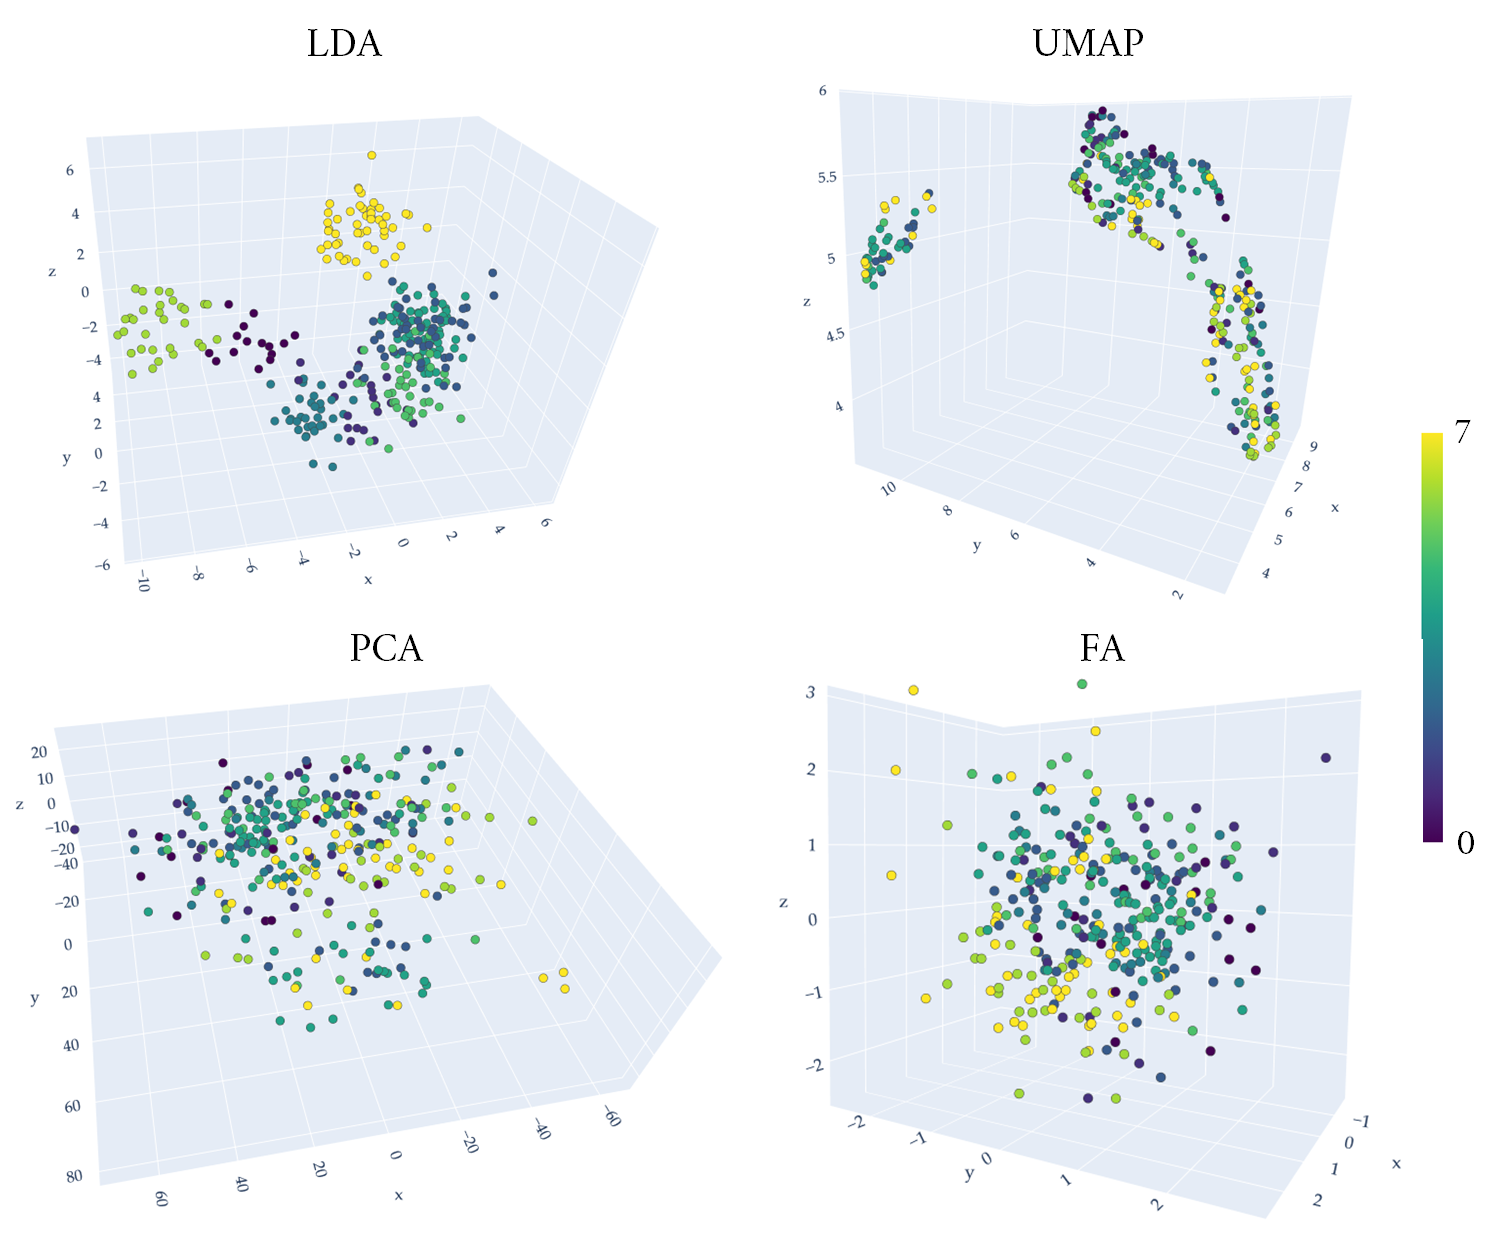
\includegraphics[width=\linewidth]{figs/vineyard_classification/feature_reduction.png}
	\caption{Feature transformation of hyperspectral data from a spectrometer using \acrshort{lda}, Uniform Manifold Approximation and Projection (\acrshort{umap}) \cite{mcinnes_umap_2020}, \acrshort{pca} and Factor Analysis (\acrshort{fa}).  }
	\label{fig:feature_reduction_spectrometer}
\end{figure}

Instead of projecting features into another space, these can be narrowed into the subset with maximum variance according to the classification labels of \acrshort{hsi} samples. There are many techniques in this field, including the Successive Projection Algorithm (\acrshort{spa}), which reduces colinearity in the feature vector. The Competitive Adaptive Reweighted Sampling (\acrshort{cars}) method selects features with Monte-Carlo sampling and iteratively removes those with small absolute regression coefficients. Two-Dimensional Correlation Spectroscopy (\acrshort{2dcs}) aims to characterize the similarity of variance in reflectance intensity. Liu et al. \cite{liu_dimension_2019} used the Ruck sensitivity analysis to discard bands with a value below a certain threshold. Agilandeeswari et al. \cite{agilandeeswari_crop_2022} calculated the band entropy, vegetation index, and water index for wavelength subsets, generating a narrower cube only with bands above three different thresholds. Finally, the work of Santos-Rufo et al. \cite{santos-rufo_wavelength_2020} presents an in-depth evaluation of methods based on Partial Least Squares (\acrshort{pls}) regression. To this end, \acrshort{hsi} data from olive orchards were first narrowed and then classified with \acrshort{lda} and \acrshort{knn}. In conclusion, the Lasso method \cite{friedman_regularization_2010} as well as Genetic algorithms \cite{mehmood_review_2012} showed the best performance with \acrshort{lda}. 

Remote sensing data typically contains inherent noise, which means it is rarely used as-is. To address this issue, Gutiérrez et al. \cite{gutierrez_--go_2018} used a combination of Standard Normal Variate (\acrshort{snv}) and de-trending to remove the scatter effect. The hyperspectral signature was then smoothed by applying the Savitzky-Golay filtering with different step sizes over the first and second derivatives.

\subsubsection{Classification of \acrshort{hsi} with \acrshort{ml} and \acrshort{dl}}

This section focuses on reviewing studies related to the classification of vineyard varieties using \acrshort{hsi}. Although there are numerous studies on \acrshort{hsi} classification, only those relevant to vineyard varieties will be discussed. In addition, state-of-the-art \acrshort{dl} networks achieving high accuracy in \acrshort{hsi} classification will also be briefly reviewed.

Despite there exists considerable research on segmentation, only a few studies have addressed the classification of vineyard varieties using \acrshort{rgb} and multispectral imagery. In these studies, binary masks or grayscale maps were first extracted to distinguish soil, shadows, and vineyards. Clustering, line detection, or \acrshort{ml} algorithms and artificial neural networks (\acrshort{ann}) were then applied to segment vineyard rows \cite{fuentes-penailillo_using_2018, karatzinis_towards_2020, hajjar_vine_2021, padua_monitoring_2020, padua_vineyard_2022, poblete-echeverria_detection_2017}. Geometrical information from depth maps, \acrshort{dem}s, \acrshort{lidar} data, and photogrammetric reconstructions were also assessed \cite{kerkech_vine_2020, aguiar_localization_2022, jurado_automatic_2020}. \acrshort{dl} approaches for semantic segmentation and skeletonization algorithms were also discussed \cite{kerkech_vine_2020-1, barros_multispectral_2022, nolan_automated_2015}. Further insight into this field is provided in \cite{li_performance_2020}. 

The classification of different vineyard varieties has been previously achieved with traditional methods and proximal hyperspectral sensing. Samples were selected by averaging the signature of each grapevine variety and keeping those with a high correlation to such a signature. Support Vector Machine (\acrshort{svm}) and Multilayer Perceptron (\acrshort{mlp}) were then trained with k-fold to distinguish thirty varieties, with the latter obtaining better results. Kicherer et al. \cite{kicherer_phenoliner_2017} presented a land phenotyping platform that segments grapes from the depth map and discerns between sprayed and non-sprayed leaves. To this end, several learning models were tested: \acrshort{lda}, Partially Least Square (\acrshort{pls}), Radial Basis Function (\acrshort{rbf}), \acrshort{mlp} and softmax output layer, with \acrshort{rbf} and \acrshort{pls} showing the best results. Besides phenotyping, the detection of plant diseases \cite{nguyen_early_2021, bendel_detection_2020, bendel_evaluating_2020} and plagues \cite{mendes_vineinspector_2022, teixeira_systematic_2023} are also recurrent research topics. However, these applications formulate a binary problem where signatures of distinct classes are significantly different regarding scale \cite{bendel_detection_2020} and shape \cite{bendel_detection_2020}. Despite this, previous learning models are also implemented (\acrshort{mlp}, \acrshort{rbf}, \acrshort{pls} and \acrshort{lda}) and almost achieved the perfect discrimination performance \cite{bendel_evaluating_2020}. Nguyen et al. \cite{nguyen_early_2021} conducted a study similar to ours, where they attempted to differentiate healthy and infected leaves with a comparable spectral signature. However, their data was obtained from land, and they used the flattened layer of 2D and 3D convolutional networks as input for Random Forest (\acrshort{rf}) and \acrshort{svm} algorithms. They found that combining \acrshort{pca} reduction (50 features) and \acrshort{rf} resulted in the best performance (97\%), and \acrshort{rf} improved \acrshort{svm} classification regardless of data reduction. Additionally, \acrshort{ml} and \acrshort{dl} techniques have been extensively applied to various crops, such as maize, sugarcane, rice, and bread wheat, using both satellite and proximal imaging. Transfer learning, attention-based, and residual models are commonly used in the literature \cite{zhang_classification_2022}. A lightweight \acrshort{cnn} composed of several inception blocks was also developed to classify up to 15 plant species \cite{liu_plant_2022}. The authors compared their proposed \acrshort{cnn} model to other commonly used models for classifying \acrshort{rgb} images, including AlexNet, VGGNet, and GoogLeNet. They found that the best results were achieved using a combination of six \acrshort{rgb} and \acrshort{nir} features, with an accuracy of 94.7\%. The use of \acrshort{pca} with only six features achieved an accuracy of 88\%. Nezami et al. \cite{nezami_tree_2020} also applied a 3D \acrshort{cnn} to classify three tree species using hyperspectral and visible images as well as canopy height models, with an overall accuracy below 95\%.

When it comes to \acrshort{dl} for the classification of \acrshort{hsi}, satellite imaging is more frequent than \acrshort{uas} imaging. To this end, there exists a standard dataset over which experiments are conducted to establish a fair comparison \cite{m_grana_hyperspectral_nodate}. The top-performing models for classifying \acrshort{hsi} are discussed below according to their contributions and overall accuracy (\acrshort{oa}). Moraga and Duzgun \cite{moraga_jigsawhsi_2022} presented an Inception-based model with parallel convolutional pipelines of increasing size, achieving near-perfect classification. Chakraborty and Trehan \cite{chakraborty_spectralnet_2021} proposed the SpectralNet model, which combines wavelet decompositions with a traditional convolutional path (\acrshort{oa}: 98.59\%-100\%). Roy et al. \cite{roy_hybridsn_2020} developed HybridSN, which includes both spectral-spatial and spatial feature learning using 3D and 2D convolutional layers (\acrshort{oa}: 99.63\%-100\%). Roy et al. \cite{roy_attention-based_2021} introduced a network based on residual blocks and spectral-spatial attention modules with varying architecture (start, middle and ending ResBlock) (\acrshort{oa}: 98.77\%-99.9\%). Lastly, Xue et al. \cite{xue_attention-based_2021} presented the A-SOP module composed of matrix-wise operations that output a second-order pooling from the attention weights, after extracting the first-order features (\acrshort{oa}: 98.68\%-100\%). 

Similar to the work of Moraga and Duzgun \cite{moraga_jigsawhsi_2022}, the FSKNet model employs a combination of 2D and 3D convolutional layers with an intermediate separable convolution to reduce training latency while achieving comparable overall accuracy results. The FSKNet model achieved an OA above 99\% with significantly fewer parameters and a shorter training time. Most of the revised work performs single-output classification, where the output is either hot-encoded or given as a single value. However, other approaches have gained attention, such as contrastive learning and multi-instance segmentation, which propose outputs of higher dimensionality. Zhu et al. \cite{zhu_spectral-spatial-dependent_2021} investigated pixel-wise semantic segmentation of \acrshort{hsi} patches using the popular U-Net architecture with additional convolutional Long Short-Term Memory (\acrshort{lstm}) and attention-based mechanisms. Xin et al. \cite{xin_convolution_2022} used transformers to independently encode spatial and spectral features and then combine them. Contrastive learning has also been used to address the lack of labelled datasets, where \acrshort{hsi} patches and 1D data are jointly used during training so that the network learns by comparing pairs of samples \cite{guan_spatial-spectral_2022}. Finally, Meerdink et al. \cite{meerdink_multitarget_2022} accurately labelled \acrshort{hsi} with multi-instance learning by creating bags of samples with distinct labels.

\subsection{Inspection of archaeological remains}

\acrshort{uas}s have been widely applied in archaeological fieldwork during the last decade \cite{campana_drones_2017}, and their products have been long studied for analyzing archaeological landscapes \cite{waagen_new_2019}. Among them, the results of \acrshort{uas} can be used to generate orthophotos and \acrshort{dem} that facilitate the observation of archaeological marks and microreliefs as proxy indicators of the presence of buried remains \cite{pecci_archaeology_2016, dubbini_digital_2016}. Furthermore, the archaeological remains are frequently located in natural landscapes barely accessible by humans with irregular features. As a result, \acrshort{uas}-based solutions have been applied to 3D reconstructions as an efficient technology that covers large and inaccessible areas. 

The preservation of cultural heritage has recently benefited from the use of high-resolution digital cameras that allow the reconstruction of a scenario with high precision. Aerial images acquired from drones not only allow us to generate 3D models using photogrammetric and \acrshort{sfm} techniques but also to obtain information beyond the visible range depending on the coupled sensors. Aerial thermographic imaging has been extensively studied in archaeology as an alternative to visible sensors \cite{casana_archaeological_2017, brooke_thermal_2018, mcleester_detecting_2018, salgado_carmona_assessing_2020}, since it allows recording the radiation emitted from object surfaces, either it proceeds from the object itself or surrounding objects \cite{vollmer_infrared_2017}. Therefore, it is possible to detect buried archaeological remains through thermal imagery whether heat transfer occurs \cite{casana_archaeological_2017}. Nevertheless, their detection is enhanced if (1) there exists a significant thermal contrast between the background and relevant features, (2) the \acrshort{uas} flight is performed at specific day intervals where the contrast of ambient temperature and sunlight radiation is higher (Figure \ref{fig:thermal_exchanging}), and (3), buried features are close to the surface. Despite thermal orthomosaics being mostly sufficient to reveal artefacts \cite{mcleester_detecting_2018, salgado_carmona_assessing_2020}, the visualization and understanding of the scene can be improved with 3D reconstructions. 

\begin{figure}[ht]
    \centering
    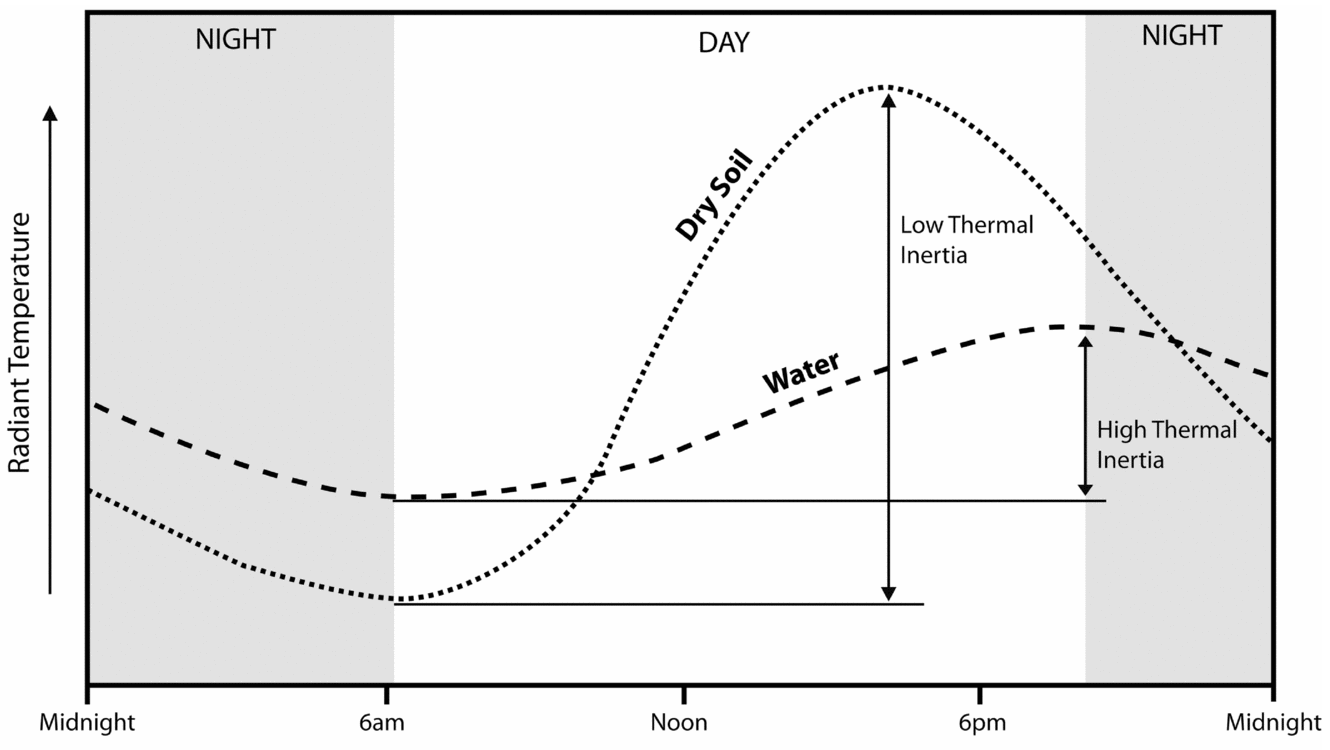
\includegraphics[width=\linewidth]{figs/castle_puerta_arenas/thermal_exchanging_day.png}
	\caption{Variation of ground and vegetation temperature over time, thus showing which is the best time of the day for collecting thermal imagery (maximum difference among both plots) \cite{casana_archaeological_2017}.}
	\label{fig:thermal_exchanging}
\end{figure}

However, consumer-grade thermal cameras present low resolution (typically $640 \times 512$ or $640 \times 480$ pixels) that limits the capability of conventional photogrammetry to generate dense and large thermal point clouds required to analyze the archaeological site \cite{javadnejad_photogrammetric_2020}. Previous work has achieved the fusion of thermography and 3D data, either from \acrshort{lidar} or photogrammetry \cite{patrucco_3d_2022}, though it has been mainly achieved in close-range inspections and façades. In contrast to thermal imagery, visible sensors acquire images of higher resolution, enabling the estimation of larger and more dense point clouds. Accordingly, \acrshort{rgb} point clouds can be used as a constrained data source to map thermographic information, thus taking advantage of their spatial characteristics. For that purpose, the relative difference between visible and thermal imaging sensors needs to be estimated in order to project 3D points into \acrshort{ir} images. The calibration of both sensors can be performed before the flight, by detecting key points in checkerboards or similar patterns \cite{adan_towards_2020, javadnejad_photogrammetric_2020}, or afterwards, by registering co-acquired images \cite{javadnejad_photogrammetric_2020}. Although multiple projection algorithms are described in the literature, these outperform others based on the \acrshort{icp} \cite{webster_three-dimensional_2018} or simply on \acrshort{sfm} reconstruction \cite{gonzalez_thermal_2019, grechi_3d_2021}, both in terms of precision and density. 






